\documentclass[twoside,11pt]{article}

% ---------------------------------------------------------------------------
% DMLR submission built on the official style file:
%   https://github.com/JmlrOrg/dmlr-style-file  (dmlr2e.sty, unmodified)
%
% DMLR uses SINGLE-BLIND review: real author names and affiliations go in
% the submission (unlike TMLR, which is double-blind).
%
% Options for dmlr2e:  abbrvbib | nohyperref | preprint
%   - Submission / review:   \usepackage[preprint]{dmlr2e}   (no Editor line, no journal/dates header)
%   - Camera-ready:          \usepackage{dmlr2e}   (fill \editor, \dmlrheading, \openreview)
% ---------------------------------------------------------------------------
\usepackage[preprint]{dmlr2e}  % preprint = review version: hides "Editor:" line and the journal/dates header. Remove [preprint] for camera-ready.

% Extra packages go AFTER dmlr2e.
% \usepackage[T1]{fontenc}  % enable only if cm-super or lmodern is installed (otherwise bitmap Type 3 fonts)
\usepackage[utf8]{inputenc}
\usepackage{amsmath}
\usepackage{booktabs}
\usepackage{adjustbox}
\usepackage{float}
% Let tall floats share a page with text instead of taking a float page of their own.
\renewcommand{\topfraction}{0.9}
\renewcommand{\bottomfraction}{0.9}
\renewcommand{\textfraction}{0.07}
\renewcommand{\floatpagefraction}{0.85}
\setcounter{topnumber}{3}
\setcounter{totalnumber}{4}
\usepackage{array}
\usepackage{xcolor}
\usepackage{lastpage}
\usepackage{url}
\def\UrlBreaks{\do\/\do-\do_\do.}
\emergencystretch=3em
\raggedbottom

% Heading arguments: {volume}{year}{pages}{date submitted}{date published}{paper id}{author full names}
% Leave as placeholders at submission time; the editorial office fills these in at acceptance.
\dmlrheading{1}{2026}{1-\pageref{LastPage}}{MM/26}{MM/26}{XX-XXXX}{Hasan Aljabbouli, Yashdeep Prasad and Bhumika Dinesh Shetty}

% Link to the OpenReview forum (required by the title block; replace once the submission exists).
\def\openreview{\url{https://openreview.net/forum?id=XXXX}}

% Running heads: {short title}{author surnames}
\ShortHeadings{LLM Formulas vs.\ Per-Row Judgments in Tabular Feature Engineering}{Aljabbouli, Prasad and Shetty}
\firstpageno{1}

\begin{document}

\title{What Actually Helps in LLM Tabular Feature Engineering?\\
A Controlled Decomposition of Deterministic Formulas\\ vs.\ Per-Row Judgments}

% Author order: Aljabbouli, Prasad, Shetty.
\author{\name Hasan Aljabbouli \email ha2285@nyu.edu \\
       \addr Department of Computer Science, Courant Institute of Mathematical Sciences\\
       New York University\\
       New York, NY 10012, USA
       \AND
       \name Yashdeep Prasad \email yp2693@nyu.edu \\
       \addr Department of Electrical and Computer Engineering\\
       New York University, Tandon School of Engineering\\
       Brooklyn, NY 11201, USA
       \AND
       \name Bhumika Dinesh Shetty \email bds9746@nyu.edu \\
       \addr Department of Electrical and Computer Engineering\\
       New York University, Tandon School of Engineering\\
       Brooklyn, NY 11201, USA}

\editor{Unassigned}

\maketitle

\begin{abstract}%
Large language models (LLMs) increasingly engineer tabular features, but deployed systems bundle mechanisms, obscuring what carries signal. We isolate two, schema-level deterministic formulas and per-row judgments, on 49 OpenML classification datasets, four schema-generating LLMs, and four downstream models (logistic regression, LR; \(k\)-nearest neighbors, KNN; random forest, RF; XGBoost). The central result is a semantic control: LLM formulas beat the same materialized features with each generated column independently permuted across rows. It is significant after Holm correction for all four models (mean ROC-AUC \(\Delta\): LR \(+0.014\), 47 of 49 datasets positive; KNN \(+0.051\), 48 of 49; RF \(+0.009\) and XGBoost \(+0.008\)) and every generator. It survives column anonymization and a six-dataset replication on real post-cutoff tables. Count-matched random valid expressions over the same columns reproduce much of this gap (three fifths for LR, three quarters for KNN), so the permutation control certifies alignment, not the generator's choices. LLM formulas still beat them for LR (\(+0.006\)), KNN (\(+0.014\)), and RF (\(+0.004\)), not XGBoost. Direct gains over raw features are small (LR \(+0.010\), KNN \(+0.007\)), absent for tree ensembles, and concentrated where raw LR trails gradient boosting. OpenFE, a search-based baseline, matches the LLM formulas for LR and is at least as good for KNN; our contribution is the decomposition, not a state-of-the-art generator. On ten core datasets with two judgment models, per-row judgments add nothing beyond zero-inference-cost formulas.

\end{abstract}

\begin{keywords}
  data-centric machine learning, tabular data, automated feature engineering, large language models, benchmark design, evaluation methodology, permutation controls, data contamination, dataset provenance
\end{keywords}

\section{Introduction}\label{sec:intro}

Feature engineering matters for tabular prediction: a few ratios, thresholds, or interactions can change the problem a downstream model sees, so recent work uses large language models (LLMs) to propose them. CAAFE has an LLM write feature code \citep{hollmann2023caafe}, FeatLLM parses LLM rules into binary features \citep{han2024featllm}, and others serialize rows as text for direct prediction \citep{hegselmann2023tabllm} or optimize feature programs with LLMs \citep{abhyankar2026llmfe,nam2024octree}. From a data-centric perspective, all of these systems are automated data-preparation tools: they change the feature representation that a downstream model sees, and their value should be measured with the same care as any other change to the data.

Two mechanisms are easy to conflate. A schema-level call writes deterministic formulas such as ratios or indicators once, at no per-row inference cost. An instance-level call reads each row and emits a judgment: flexible but expensive, slow, and hard to audit.

We ask whether LLM-generated formulas carry real semantic signal or merely add columns, and whether per-row judgments add anything beyond them. These are benchmarking questions about a data-preparation step: the object under evaluation is the feature representation, the unit of analysis is the dataset, and each control holds the data fixed except for the property under test, following the data-centric view that benchmarks data preparation itself \citep{zha2025datacentric,mazumder2023dataperf,tschalzev2024datacentric}. Because popular public tables are in the models' training data \citep{bordt2024elephants}, the benchmark also needs contamination controls.

The most robust result is a semantic control, not the raw-to-formula comparison: correct formula features consistently beat the same features with generated columns independently row-permuted. On 49 datasets and four schema generators it is significant after multiple-comparison correction for all four downstream models, largest for logistic regression (LR) and \(k\)-nearest neighbors (KNN), smaller for tree ensembles, and present for every generator, under column anonymization, and on six post-cutoff tables. Much of this gap is generic to any valid expression over the same columns; the generator-specific remainder is small but consistent for LR and KNN, smaller for RF, and absent for XGBoost. Direct gains over raw features are small and model-dependent, no generator, LLM or classical automated feature engineering (AutoFE), helps tree ensembles, and per-row judgments add essentially nothing beyond formulas.

Contributions:

\begin{itemize}
\item
  A documented two-tier benchmark: 49 OpenML classification datasets (10 core, 39 expansion) with recorded identifiers, versions, and licences (Appendix~\ref{app:datasets}), evaluating schema-level formulas and per-row judgments from four generators under one protocol.
\item
  A benchmarking method for feature generators: a column-permutation control that preserves marginal distributions and feature count but breaks row alignment, paired with a count-matched random-expression control over the same columns and vocabulary (Section~\ref{sec:random-expression}).
\item
  Two contamination controls for public-table benchmarks: an anonymized-column control on the core datasets and a replication on six real datasets with provenance and licences (Appendix~\ref{app:postcutoff-data}) whose tables post-date the generators' training data (Section~\ref{sec:postcutoff}).
\item
  A negative result for per-row LLM judgments: on the ten core datasets they do not improve over zero-inference-cost deterministic formulas.
\item
  Classical AutoFE baselines (polynomial, OpenFE, autofeat) on the 49 datasets: search-based OpenFE matches the LLM formulas for LR and is at least as good for KNN; our contribution is the controlled decomposition, not a state-of-the-art generator.
\end{itemize}

\section{Related Work}\label{sec:related-work}

\paragraph{LLMs for tabular learning and feature engineering.}

LLMs serve tabular data as predictors and feature generators \citep{fang2024survey,hegselmann2023tabllm}: CAAFE, FeatLLM, and FELIX turn LLM-proposed transformations or rules into features \citep{hollmann2023caafe,han2024featllm,malberg2024felix}; later work searches over feature programs \citep{nam2024octree,abhyankar2026llmfe,gong2025evolutionary,zhang2025dynamic} or lets agents revise whole pipelines on Kaggle-derived benchmarks \citep{guo2024dsagent,hong2025datainterpreter,chi2024sela,jiang2025aide,li2024autokaggle,chan2025mlebench}. LLM generators favor simple operators at a cost in predictive performance \citep{kuken2024simple}, motivating our random-expression control over the same vocabulary (Section~\ref{sec:controls}). We isolate two mechanisms these systems bundle: deterministic formulas and per-row judgments.

\paragraph{Traditional automated feature engineering.}

Classical AutoFE builds and selects transformations without language-model semantics by composing primitives across linked tables \citep{kanter2015dfs}, searching or learning which transformations help \citep{khurana2016cognito,katz2016explorekit,nargesian2017lfe,khurana2018rl,zhu2022difer}, or filtering large candidate pools in stages \citep{horn2020autofeat,zhang2023openfe}. As they too add columns, they are natural baselines; we run polynomial interactions, OpenFE, and autofeat to completion on the same 49 datasets (Section~\ref{sec:classical}).

\paragraph{Evaluation across datasets.}

Cross-dataset comparisons use nonparametric tests, Wilcoxon signed-rank \citep{wilcoxon1945individual} for pairs and Friedman/Nemenyi \citep{friedman1937use} for rankings \citep{demsar2006statistical,garcia2010advanced}, and large benchmarks report per-dataset ranks or normalized scores rather than pooled scores \citep{grinsztajn2022tree,mcelfresh2023neural,erickson2025tabarena}. We follow suit: the dataset is the statistical unit; fold-level variation serves estimation only.

\paragraph{Permutation controls.}

Permuting labels \citep{ojala2010permutation} or single features \citep{breiman2001random,fisher2019all,altmann2010permutation,strobl2008conditional} tests for dependence on feature-label alignment rather than distributional artifacts, though unconditional test-time permutation forces extrapolation to unseen feature combinations \citep{hooker2021unrestricted}. Our control independently permutes each generated column before cross-validation, so the model is refitted on the permuted columns, not evaluated off-distribution. Beating the permuted copy rules out dimensionality, syntax, and marginal distributions as sole explanations; the random-expression control (Section~\ref{sec:controls}) asks how much of the gap any valid expression over the same columns produces.

\paragraph{Contamination and memorization in tabular LLM evaluation.}

Language models memorize training data \citep{carlini2023quantifying}, so test sets seen in pretraining inflate measured ability \citep{sainz2023nlp,xu2024benchmark}; detectors use guided completion \citep{golchin2024time} or post-cutoff problems \citep{roberts2024cutoff,white2025livebench}, and \citet{bordt2023testing,bordt2024elephants} show verbatim memorization of popular tabular datasets and higher few-shot performance on tables seen in training. We likewise use post-cutoff tables (Section~\ref{sec:postcutoff}) and anonymized schemas that hide column names and dataset identity (Section~\ref{sec:anon}); both controls are partial (Sections~\ref{sec:postcutoff} and~\ref{sec:limitations}).

\paragraph{Tabular benchmarks and data-centric evaluation.}

OpenML suites pin collections and versions \citep{vanschoren2014openml,bischl2021openml}; large comparisons show that conclusions depend on dataset population, evaluation protocol, and split design \citep{gorishniy2021revisiting,grinsztajn2022tree,mcelfresh2023neural,ye2024closer,erickson2025tabarena,rubachev2025tabred}. \citet{tschalzev2024datacentric} argue that dataset-specific feature engineering changes model rankings and belongs in the benchmark, as data-centric AI \citep{zha2025datacentric,liang2022advances} and DataPerf \citep{mazumder2023dataperf} do for data preparation; datasheets \citep{gebru2021datasheets} set the documentation standard of Appendices~\ref{app:datasets} and~\ref{app:postcutoff-data}. We treat LLM feature generation the same way: the benchmark is pinned to OpenML identifiers, versions, and licences, and each control varies one property.

\section{Evaluation Pipeline and Controls}\label{sec:method-the-dasef-pipeline}

The DASEF (Downstream-Aware Semantic Feature Engineering) pipeline (Figure~\ref{fig:pipeline}) has four steps: a schema-level LLM call on a column summary, formula materialization, optional per-row judgments, and count-matched and row-permutation controls scored with every schema run.

\begin{figure}[tbp]
\centering
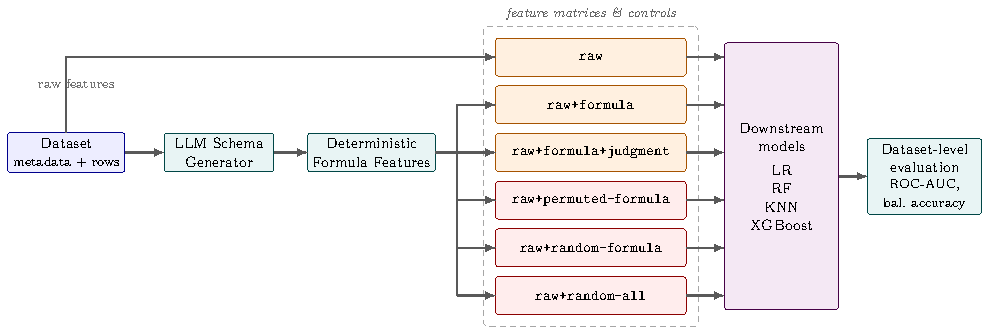
\includegraphics[width=\linewidth]{figures/fig1_pipeline.pdf}
\caption{Overview of the DASEF evaluation pipeline. Schema-level LLM calls generate deterministic formulas once per dataset; downstream evaluation compares raw features, formula features, optional per-row judgments, and controls that preserve feature count while removing semantic alignment. The count-matched random-expression control of Section~\ref{sec:controls} is evaluated alongside these matrices (not shown); the generator receives only the column-level summary of the design split, never rows.}\label{fig:pipeline}
\end{figure}


\subsection{Schema-level formula generation}\label{sec:schema-level-formula-generation}

For each dataset, a schema generator receives a column-level summary of a schema-design split: column names, dtypes, missing rates, mean/std/min/max for numeric columns or the ten most frequent values for categorical ones, and the class balance. No rows or row-level labels are sent. It returns a fixed schema of 12 features: deterministic formulas plus per-row judgment specifications (counts in Appendix~\ref{app:protocol-details}). Formulas are then applied to the evaluation rows without further LLM calls.

Four generators were evaluated: Claude Opus 4.7, Claude Sonnet 4.6, Gemini 3.1 Pro Preview, and GPT-5.5 Pro, each prompted for three model families: linear and support-vector-machine (linear/SVM), tree/ensemble, and distance-based KNN. The family labels are experimental conditions, not evidence of specialization: a downstream-awareness diagnostic on the core tier finds no reliable matched-family advantage (Section~\ref{sec:discussion}). Benchmark-wide analyses therefore use each generator's linear/SVM schema, averaged over the generators covering a dataset before testing; the core tier has all three families from all four generators (Appendix~\ref{app:core-families}).

\subsection{Per-row judgment generation}\label{sec:judgment}

The second component appends row-level LLM judgments, intended to capture what deterministic formulas cannot express. Judgments are the expensive component, since they need row-level LLM calls, and are harder to reproduce and audit, so their value is assessed only incrementally: \texttt{raw+formula} versus \texttt{raw+formula+judgment}. DeepSeek-Reasoner produced them in 25-row batches for all 120 core runs; Appendix~\ref{app:judgment-v4pro} reports a second judgment model, and the expansion tier has none (Appendix~\ref{app:protocol-details}).

\subsection{Controls}\label{sec:controls}

\paragraph{Column-permuted formula control.}

The strongest control keeps the materialized formula features but independently permutes each generated column across evaluation rows. This preserves the feature count and each column's exact marginal distribution but breaks row alignment; a column with row-aligned structure should beat its permuted copy. It tests row-aligned signal in the materialized feature, not whether the LLM invented it. Each column is permuted once over the whole evaluation split (seed 42) before cross-validation, so training and test folds are permuted jointly. Scoring uses the same folds, fold by fold, with one draw per schema run.

\paragraph{Random feature control.}

Random controls add uniform-noise columns (seeds 42 and 43) matched in count and declared value range (Appendix~\ref{app:protocol-details}) to the formula features (\texttt{raw+random-formula}) or to all schema features, judgment specifications included (\texttt{raw+random-all}). They test whether arbitrary added columns suffice, and are less stringent than permutation because they do not preserve formula syntax.

\paragraph{Random-expression control.}

For every (dataset, generator) cell of the linear/SVM benchmark, this control draws \(k\) random but valid expressions over the dataset's own columns from the vocabulary of the LLM formulas, with \(k\) the number of formula features in the cell's LLM schema and only design-split column statistics as input; five independent draws per cell are scored and averaged. Materialization, range clipping, folds, downstream models, and column permutation match the LLM formulas (Appendix~\ref{app:protocol-details}). It asks whether random valid expressions help over \texttt{raw}, how much of the aligned-versus-permuted gap they reproduce, and whether the LLM's choices beat random choices of the same size and vocabulary (\texttt{raw+formula} versus \texttt{raw+random-expression}; Section~\ref{sec:random-expression}).

\subsection{Evaluation protocol}\label{sec:protocol}

Datasets above 5,000 rows are capped to a stratified 5,000-row sample (seed 42). A stratified 30\% schema-design split follows (seed 42), and the remaining 70\% are the evaluation rows: 3,500 for capped datasets, 524 to 3,783 otherwise. Scores use 5-fold cross-validation (CV) with 2 repeats. The downstream models are logistic regression (LR; class-balanced, up to 2,000 iterations), random forest (RF; 300 trees, \(\sqrt{p}\) candidate features per split, balanced-subsample class weights), \(k\)-nearest neighbors (KNN; \(k = 15\)), and XGBoost \citep{chen2016xgboost} (300 trees, depth 4, learning rate 0.05, 0.9 row and column subsampling), with library defaults otherwise. Numeric columns are median-imputed and, for LR and KNN, standardized; categorical columns are mode-imputed and one-hot encoded. Six core datasets (adult income, bank marketing, car evaluation, electricity, phoneme, spambase) come from a local cache; in three of them (adult income, bank marketing, car evaluation) it stores the categorical columns as integer codes. The schema generators therefore saw these columns as integers and their formulas compute on the codes; before downstream modelling the columns are restored to categoricals, so the raw block is one-hot encoded as for every other dataset (Appendix~\ref{app:protocol-details}). The primary metric is one-vs-rest ROC-AUC, macro-averaged over classes for the 12 multiclass datasets; balanced accuracy is secondary.

On both tiers the schema summaries came from design splits of the full, uncapped dataset, so on capped datasets they also cover later evaluation rows. Only distributional statistics and the class balance were exposed, never row-level labels; Section~\ref{sec:leakage} bounds the effect (Appendix~\ref{app:protocol-details}).

Matrix variants:

\begin{itemize}
\item
  \texttt{raw}: preprocessed original features.
\item
  \texttt{raw+formula}: plus the LLM formulas.
\item
  \texttt{raw+formula+judgment}: plus per-row judgments (core tier only).
\item
  \texttt{raw+permuted-formula}: plus the formulas with each generated column row-permuted.
\item
  \texttt{raw+random-formula}: plus uniform noise count- and range-matched to the formulas.
\item
  \texttt{raw+random-all}: plus uniform noise matched to all schema features.
\item
  \texttt{raw+random-expression}: plus count-matched random valid expressions (linear/SVM cells only), also scored permuted.
\end{itemize}

\subsection{Statistical analysis}\label{sec:statistical-analysis}

The statistical unit is the dataset. For each dataset, downstream model, metric, and matrix pair, fold-level scores are averaged within each schema run, then over the generators covering the dataset (four for 34 of the 49 datasets; Section~\ref{sec:datasets}); paired differences are then taken per dataset. Paired \(p\)-values are exact two-sided Wilcoxon signed-rank tests over the dataset-level differences, ties excluded, with Holm-Bonferroni correction over the four downstream models (family size four, within each metric and contrast) reported alongside. Cliff's \(\delta\) is the one-sample form \((wins - losses)/N\) against zero; 95\% confidence intervals (CI) for mean differences are percentile bootstrap intervals over datasets (10,000 resamples). Rankings use the Friedman test with the Nemenyi post-hoc critical difference \citep{demsar2006statistical}. Core-tier-only analyses (per-row judgments, schema families, the anonymized control) have ten datasets and sit at the Wilcoxon floor, where the smallest attainable two-sided \(p\) is \(0.002\) for a 10/10 sweep; they are reported uncorrected as supporting evidence. A global Benjamini-Hochberg check over all 48 tests of Tables~\ref{tab:semantic-direct} and~\ref{tab:random-expression} leaves every cell reported as significant below \(q = 0.05\); Appendix~\ref{app:protocol-details} gives the Holm-over-48 picture.

The contrasts are

\begin{align}
\Delta_{\mathrm{formula}}  &= s(\texttt{raw+formula}) - s(\texttt{raw}), \label{eq:formula}\\
\Delta_{\mathrm{judgment}} &= s(\texttt{raw+formula+judgment}) - s(\texttt{raw+formula}), \label{eq:judgment}\\
\Delta_{\mathrm{semantic}} &= s(\texttt{raw+formula}) - s(\texttt{raw+permuted-formula}), \label{eq:semantic}
\end{align}

where \(s( \cdot )\) is the cross-validated score for a fixed dataset, downstream model, and metric. The main claim is about \(\Delta_{\mathrm{semantic}}\), not \(\Delta_{\mathrm{formula}}\): a feature can encode real semantic structure yet not improve a high-capacity model over raw inputs.

\section{Benchmark Construction and Experimental Setup}\label{sec:experimental-setup}

\subsection{Datasets: a two-tier benchmark}\label{sec:datasets}

The two tiers are listed in Appendix~\ref{app:datasets} (Table~\ref{tab:datasets}).

\paragraph{Core tier (10 datasets).}

Ten OpenML \citep{vanschoren2014openml} classification datasets span low-feature medical and behavioral, categorical symbolic, business and socioeconomic, signal-processing, and higher-dimensional numeric/text-derived tasks: adult income, bank marketing, blood transfusion, car evaluation, credit-g, electricity, phoneme, pima diabetes, QSAR biodegradation, and spambase. Every core dataset has schemas from all four generators and all three families (12 schema runs), per-row judgment matrices, and the anonymized-column control. Three of the six locally cached core datasets (Section~\ref{sec:protocol}) are variants of the listed OpenML table: bank marketing is the 20-feature, 41,188-row UCI bank-additional variant rather than the 16-feature OpenML 1461 version, electricity is a 7-feature, 38,474-row variant of OpenML 151 without the \texttt{day} column, and adult income is the 45,222-row complete-case version of OpenML 1590.

\paragraph{Expansion tier (39 datasets).}

The expansion tier adds every dataset from a pool of 42 further OpenML classification datasets, configured for a planned larger study, with a valid cached linear/SVM-family schema from at least one generator and a successful stratified 30/70 split. Three are excluded: \texttt{advanced\_iot\_dataset} and \texttt{letter}, where every generator response failed validation, and \texttt{nursery}, whose single-member class the stratified split rejects. Each expansion dataset has the linear/SVM schema of every generator that produced one: 24 of the 39 are covered by all four generators, seven by three, six by two, and two by one (Gen.\ column of Table~\ref{tab:datasets}). This tier has no judgment features and only the linear/SVM family, so judgment, family, and anonymization analyses use the core tier only and formula-mechanism analyses all 49 datasets. In 13 schema cells on seven datasets whose column names are not valid Python identifiers, the generator saw column names sanitized to valid identifiers, and the same renaming is applied to the evaluation rows before materialization (Appendix~\ref{app:provenance} lists the cells).

\subsection{Scale of evaluation}\label{sec:scale-of-evaluation}

The formula evaluation covers 251 schema runs, 120 on the core tier (4 generators \(\times\) 3 families \(\times\) 10 datasets) and 131 on the expansion tier, each with five matrix variants (six on the core tier, where the judgment matrix is added), four downstream models, and 5-fold \(\times\) 2-repeat cross-validation, roughly 55,000 fold-level downstream evaluations; the random-expression control adds two matrices for each of five random draws in each of the 171 linear/SVM cells, a further 68,400. Each schema run is one generator call cached by prompt hash; the expansion schemas were evaluated offline from that cache, so no schema was selected or edited after its evaluation was known. The judgment columns alone reach ROC-AUC 0.66 with logistic regression, so they carry signal; Section~\ref{sec:per-row-judgments-add-no-reliable-value-beyond-formulas} shows this signal is redundant with \texttt{raw+formula}. Appendix~\ref{app:provenance} reports the judgment audit, response accounting, truncated schemas, and a constant-column scan.

\subsection{Prospective versus cached schema generation}\label{sec:leakage}

Schemas were generated from design-split summaries of the uncapped table, so on capped datasets of both tiers the summarized rows overlap the evaluation rows (Section~\ref{sec:protocol}). A leakage-equivalence check bounds this overlap: on 54 overlapping cells, the raw-to-formula deltas from cached and prospective evaluation of the same schemas differ by 0.0050 in mean absolute value and by \(+0.0023\) signed (cached minus prospective; Appendix~\ref{app:provenance}).

\subsection{Reproducibility}\label{sec:reproducibility}

Random seeds are 42 for the row cap, the design split, cross-validation, and permutations, and 43 for the random-all control. Checked-in scripts regenerate the classical baselines (Section~\ref{sec:classical}), the mechanism case study (Appendix~\ref{app:mechanism}), every control, and every aggregate, table, and figure offline from the cached schemas and stored matrices. Table~\ref{tab:models} (Appendix~\ref{app:provenance}) lists generator API identifiers, settings, and query dates, and the appendix records compute. A final audit found and fixed three formula-evaluator defects (a column named like a numpy function was shadowed by that function, \texttt{category}-typed columns were coerced so that string comparisons or arithmetic on them became silently constant, and narrow integer columns overflowed inside sums and products); every stored run was re-materialized and affected runs re-evaluated with the corrected evaluator, which produced every number reported here.

\paragraph{Data and code availability.}

Code, cached schemas and raw generator responses, per-fold scores, the benchmark definition, per-dataset provenance records (\texttt{dataset\_provenance.csv}), and the scripts regenerating every table and figure are in the supplementary material and at \url{https://github.com/prasad-yashdeep/dasef-tabular-research} (release \texttt{v1.1-dmlr-submission}); the stored feature matrices and the per-row judgment outputs are release assets there. Code is released under the MIT licence and derived artifacts (schemas, responses, scores, statistics, generated columns) under CC BY 4.0, except that artifacts derived from the two CC BY-NC post-cutoff tables carry the same non-commercial restriction; raw dataset columns embedded in the released matrices and the cached tables remain under their sources' terms. A datasheet-style description accompanies the supplement; the intended use is controlled evaluation of feature-generation tools for tabular classification under the controls of Section~\ref{sec:controls}, not training deployed models on the generated features. Appendix~\ref{app:provenance} covers table licences and maintenance.

\section{Results}\label{sec:results}

\subsection{Formula features encode semantic structure}\label{sec:semantic}

Across the 49 datasets, correct formulas beat their column-permuted copies for every downstream model (Table~\ref{tab:semantic-direct}, Figure~\ref{fig:semantic-dotplot}). For ROC-AUC the effect is largest for the capacity-limited models: LR \(+0.0140\) (47/1, \(p = 2 \times 10^{-13}\), 95\% CI \(\lbrack +0.009, +0.019\rbrack\)) and KNN \(+0.0510\) (48/1, \(p = 2 \times 10^{-13}\), CI \(\lbrack +0.040, +0.064\rbrack\)). It is smaller but significant for the tree ensembles: RF \(+0.0085\) (30/17, \(p = 0.003\), CI \(\lbrack +0.003, +0.016\rbrack\)) and XGBoost \(+0.0085\) (39/7, \(p = 2 \times 10^{-6}\), CI \(\lbrack +0.004, +0.014\rbrack\)). All four cells survive Holm correction, and balanced accuracy is significant for all four models with at least 40 wins each. Medians are well below the means (LR \(+0.0051\), KNN \(+0.0428\), RF \(+0.0010\), XGBoost \(+0.0025\)), so a minority of datasets carries the mean upward. The semantic delta is negative in 5\% of (dataset, generator) cells for LR, 4\% for KNN, 17\% for XGBoost, and 28\% for RF, which is negative on 17 of the 49 datasets; without its largest effect (employee turnover, \(+0.142\)) the RF mean is \(+0.006\) (29/17, \(p = 0.005\)).


\begin{table}[tbp]
\caption{Semantic control and direct effect of LLM formulas on all 49 datasets (generator-averaged linear/SVM schemas). ``Semantic $\Delta$'' is \texttt{raw+formula} minus \texttt{raw+permuted-formula}; ``Direct $\Delta$'' is \texttt{raw+formula} minus \texttt{raw}. $p$ is the exact two-sided Wilcoxon signed-rank test over datasets (ties excluded from W/L); $p_{\mathrm{Holm}}$ corrects over the four downstream models within each metric and contrast.}\label{tab:semantic-direct}
\centering
\small
\begin{adjustbox}{max width=\linewidth}
\begin{tabular}{llrrrrrrrrr}
\toprule
Metric & Downstream model & \(N\) & Semantic \(\Delta\) & W/L & \(p\) & \(p_{\mathrm{Holm}}\) & Direct \(\Delta\) & W/L & \(p\) & \(p_{\mathrm{Holm}}\) \\
\midrule
ROC-AUC & Logistic regression & 49 & +0.0140 & 47/1 & $<$0.001 & $<$0.001 & +0.0096 & 35/13 & $<$0.001 & $<$0.001 \\
ROC-AUC & KNN & 49 & +0.0510 & 48/1 & $<$0.001 & $<$0.001 & +0.0067 & 29/20 & 0.014 & 0.042 \\
ROC-AUC & Random forest & 49 & +0.0085 & 30/17 & 0.003 & 0.003 & +0.0019 & 21/26 & 0.386 & 0.772 \\
ROC-AUC & XGBoost & 49 & +0.0085 & 39/7 & $<$0.001 & $<$0.001 & -0.0000 & 18/28 & 0.516 & 0.772 \\
\midrule
Bal. accuracy & Logistic regression & 49 & +0.0165 & 44/4 & $<$0.001 & $<$0.001 & +0.0111 & 34/15 & $<$0.001 & $<$0.001 \\
Bal. accuracy & KNN & 49 & +0.0735 & 46/2 & $<$0.001 & $<$0.001 & +0.0124 & 30/18 & 0.013 & 0.038 \\
Bal. accuracy & Random forest & 49 & +0.0303 & 40/7 & $<$0.001 & $<$0.001 & +0.0076 & 28/20 & 0.016 & 0.038 \\
Bal. accuracy & XGBoost & 49 & +0.0137 & 41/6 & $<$0.001 & $<$0.001 & +0.0018 & 22/25 & 0.492 & 0.492 \\
\bottomrule
\end{tabular}
\end{adjustbox}
\end{table}

\begin{figure}[tbp]
\centering
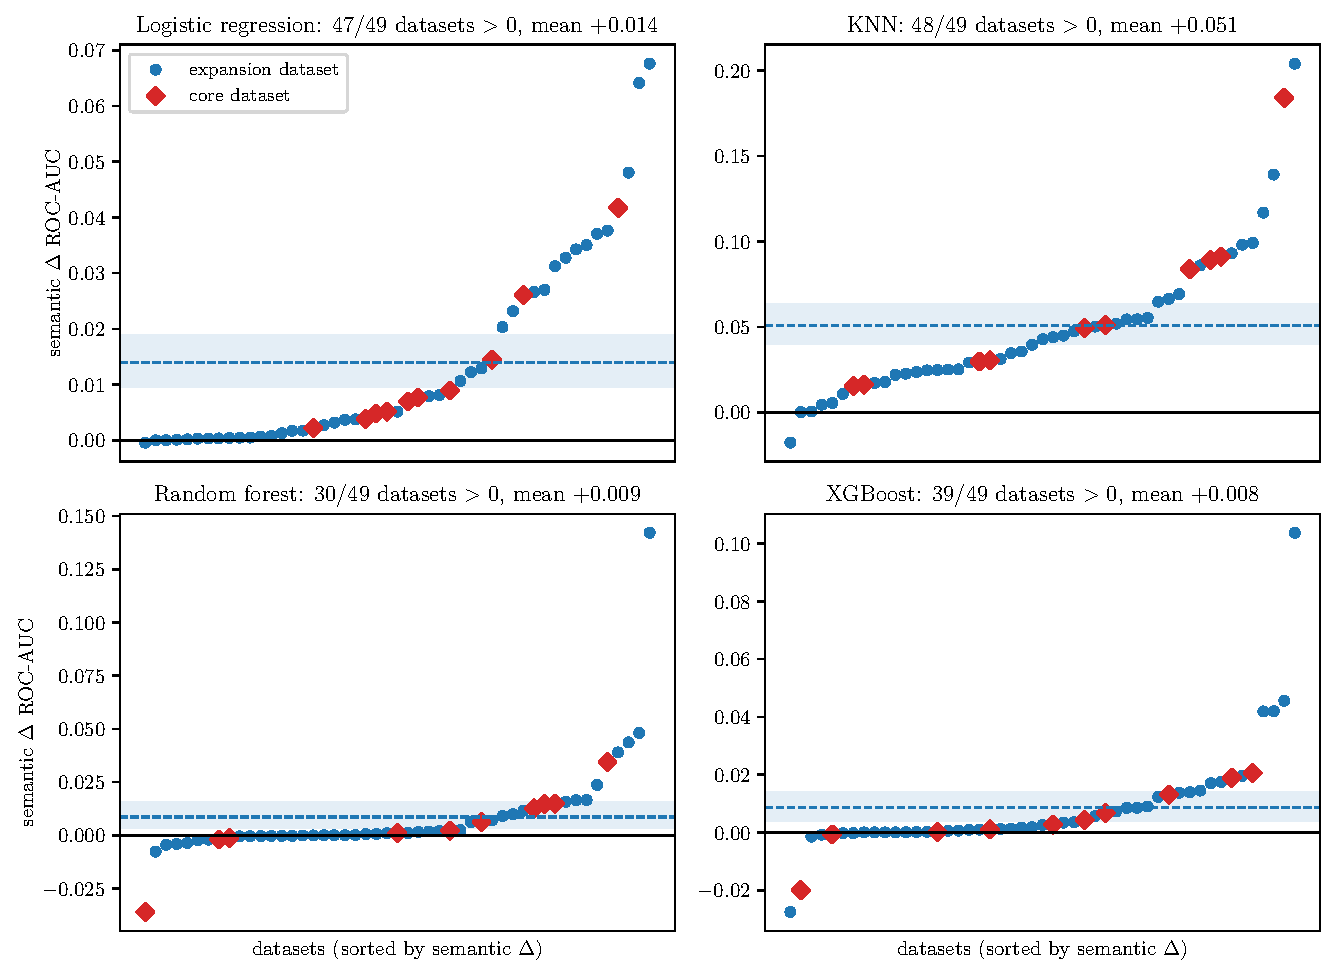
\includegraphics[width=0.92\linewidth]{figures/fig2_semantic_deltas.pdf}
\caption{Dataset-level semantic-control ROC-AUC deltas (\texttt{raw+formula} minus \texttt{raw+permuted-formula}) on all 49 datasets, one panel per downstream model, datasets sorted within each panel. Red diamonds are core datasets, blue dots expansion datasets; the dashed line is the mean and the band its 95\% bootstrap interval. The effect is positive on nearly every dataset for LR and KNN and on a clear majority for the tree ensembles.}\label{fig:semantic-dotplot}
\end{figure}


The result holds in each tier and without generator averaging. On the ten core datasets alone (linear/SVM schemas), LR and KNN are 10/0 (\(+0.012\) and \(+0.064\); nominal \(p = 0.002\)) and the tree ensembles positive in mean but not significant at \(N = 10\); on the 39 expansion datasets alone all four contrasts are significant (LR 37/1, KNN 38/1, RF 23/14 with \(p = 0.010\), XGBoost 31/5 with \(p = 5 \times 10^{-6}\)). On the 34 datasets covered by all four generators, LR is \(+0.018\) (34/0), KNN \(+0.054\) (33/1), RF \(+0.010\) and XGBoost \(+0.008\) (both \(p < 0.001\)). Each generator reproduces the pattern alone (Section~\ref{sec:generators}), as does averaging all three core-tier schema families (Appendix~\ref{app:core-families}).

Count-matched noise columns hurt every model (Table~\ref{tab:random-controls}, Appendix~\ref{app:extra-tables}), and \texttt{raw+formula} beats \texttt{raw+random-formula} for all four (LR \(+0.0134\), KNN \(+0.0541\), RF \(+0.0101\), XGBoost \(+0.0126\); Holm-corrected \(p < 0.001\)), so the gap is not a dimensionality artifact. One caveat: \(\Delta_{\mathrm{semantic}}\) is \(\Delta_{\mathrm{formula}}\) plus the harm permuted columns do relative to raw, roughly 30\% of the LR gap and most or all of the KNN, RF, and XGBoost gaps (permuted-minus-raw \(-0.044\), \(-0.007\), \(-0.009\) against direct gains \(+0.007\), \(+0.002\), \(0.000\)), so aligned columns are near-harmless and misaligned copies harmful, which shows that alignment matters but not that aligned formulas add information beyond raw features for the tree ensembles.

\subsection{How much of the semantic gap is generic? The random-expression control}\label{sec:random-expression}

Random valid expressions, the count-matched control of Section~\ref{sec:controls}, also beat their permuted copies for LR, KNN, and XGBoost (Table~\ref{tab:random-expression}; ROC-AUC: LR \(+0.0083\), 47/2; KNN \(+0.0391\), 48/1; XGBoost \(+0.0048\), 40/6; all Holm-corrected \(p < 0.001\)) and in mean for RF (\(+0.0031\), 29/18, \(p = 0.10\)). In mean this generic component is 59\% of the LLM semantic gap for LR, 77\% for KNN, 36\% for RF, and 57\% for XGBoost. The permutation control therefore certifies row alignment, not the quality of the generator's choices.

Two contrasts isolate those choices. First, random expressions add little: versus raw they help LR slightly (\(+0.0032\), 28/21, Holm-corrected \(p = 0.012\), a third of the LLM direct gain) and hurt KNN (\(-0.0068\), 9/40), RF (\(-0.0017\), 8/39), and XGBoost (\(-0.0007\), 14/32), against LLM direct gains of \(+0.0096\) (LR) and \(+0.0067\) (KNN) (Table~\ref{tab:semantic-direct}). Second, with both aligned, LLM formulas beat random expressions for LR (\(+0.0064\), 40/9, Holm-corrected \(p < 0.001\)), KNN (\(+0.0135\), 43/6, \(p < 0.001\)), and RF (\(+0.0036\), 31/16, \(p = 0.005\)), not for XGBoost (\(+0.0007\), 22/24); balanced accuracy agrees (RF \(+0.0069\), 32/16, \(p = 0.002\)). The excess semantic contrast (LLM minus random-expression) is positive and significant for all four models (\(+0.0037\) for XGBoost to \(+0.0118\) for KNN; Holm-corrected \(p < 0.001\) for LR, KNN, and RF, \(p = 0.003\) for XGBoost). The LLM-minus-random contrast holds for LR and KNN for each generator separately (uncorrected \(p \le 0.0008\) and \(p \le 0.0001\)) and on the 39 expansion datasets alone (LR \(+0.0073\), 32/7; KNN \(+0.0131\), 34/5); on the ten core datasets alone it is smaller (LR \(+0.0028\), 8/2, uncorrected \(p = 0.037\); KNN \(+0.0153\), 9/1, \(p = 0.004\)). Of the 8{,}400 random expression columns (five draws per cell), 29 were constant on the evaluation rows (15 cells); all were kept. The generator-specific signal is real but modest: about two fifths of the LLM permutation contrast for LR (\(0.0057/0.0140\)), a quarter for KNN (\(0.0118/0.0510\)), and, as a direct contrast, absent for XGBoost.


\begin{table}[tbp]
\caption{Random-expression control on all 49 datasets (ROC-AUC and balanced accuracy, generator-averaged). Each (dataset, generator) cell receives $k$ random but valid expressions over the dataset's own columns, drawn from the LLM formulas' vocabulary with design-split statistics only, where $k$ is the cell's number of LLM formula features (Section~\ref{sec:controls}); they are materialized, scored, and column-permuted exactly like the LLM formulas, and the random-expression columns of the table are averaged over five independent random schemas per cell. ``Random expr.\ $-$ raw'': \texttt{raw+random-expression} minus \texttt{raw}; ``Random expr.\ vs permuted'': random expressions minus their own permuted copy; ``LLM $-$ random expr.'': \texttt{raw+formula} minus \texttt{raw+random-expression}; ``Excess semantic'': the LLM semantic contrast of Table~\ref{tab:semantic-direct} minus the random-expression semantic contrast. W/L counts datasets (ties excluded); $p_{\mathrm{Holm}}$ is the exact Wilcoxon test over datasets, Holm-corrected over the four models.}\label{tab:random-expression}
\centering
\small
\begin{adjustbox}{max width=\linewidth}
\begin{tabular}{llrrrrrrrrrrrr}
\toprule
& & \multicolumn{3}{c}{Random expr. $-$ raw} & \multicolumn{3}{c}{Random expr. vs permuted} & \multicolumn{3}{c}{LLM $-$ random expr.} & \multicolumn{3}{c}{Excess semantic} \\
\cmidrule(lr){3-5}\cmidrule(lr){6-8}\cmidrule(lr){9-11}\cmidrule(lr){12-14}
Metric & Model & $\Delta$ & W/L & $p_{\mathrm{Holm}}$ & $\Delta$ & W/L & $p_{\mathrm{Holm}}$ & $\Delta$ & W/L & $p_{\mathrm{Holm}}$ & $\Delta$ & W/L & $p_{\mathrm{Holm}}$ \\
\midrule
ROC-AUC & Logistic regression & +0.0032 & 28/21 & 0.012 & +0.0083 & 47/2 & $<$0.001 & +0.0064 & 40/9 & $<$0.001 & +0.0057 & 39/10 & $<$0.001 \\
ROC-AUC & KNN & -0.0068 & 9/40 & $<$0.001 & +0.0391 & 48/1 & $<$0.001 & +0.0135 & 43/6 & $<$0.001 & +0.0118 & 38/11 & $<$0.001 \\
ROC-AUC & Random forest & -0.0017 & 8/39 & $<$0.001 & +0.0031 & 29/18 & 0.102 & +0.0036 & 31/16 & 0.005 & +0.0055 & 36/11 & $<$0.001 \\
ROC-AUC & XGBoost & -0.0007 & 14/32 & 0.008 & +0.0048 & 40/6 & $<$0.001 & +0.0007 & 22/24 & 0.778 & +0.0037 & 32/14 & 0.003 \\
\midrule
Bal. accuracy & Logistic regression & +0.0046 & 33/16 & 0.010 & +0.0101 & 46/3 & $<$0.001 & +0.0065 & 36/13 & 0.001 & +0.0064 & 37/12 & 0.002 \\
Bal. accuracy & KNN & -0.0094 & 10/38 & $<$0.001 & +0.0527 & 46/2 & $<$0.001 & +0.0218 & 41/7 & $<$0.001 & +0.0208 & 35/13 & $<$0.001 \\
Bal. accuracy & Random forest & +0.0007 & 19/28 & 0.183 & +0.0198 & 40/8 & $<$0.001 & +0.0069 & 32/16 & 0.002 & +0.0105 & 37/11 & $<$0.001 \\
Bal. accuracy & XGBoost & -0.0004 & 27/20 & 0.846 & +0.0093 & 42/5 & $<$0.001 & +0.0021 & 22/25 & 0.539 & +0.0044 & 33/14 & $<$0.001 \\
\bottomrule
\end{tabular}
\end{adjustbox}
\end{table}


\subsection{Direct formula gains are small and model-dependent}\label{sec:direct}

Direct gains over raw features are small and model-dependent (Table~\ref{tab:semantic-direct}, right half): LR gains \(+0.0096\) ROC-AUC (35/13, \(p = 1 \times 10^{-5}\), CI \(\lbrack +0.005, +0.015\rbrack\)) and KNN \(+0.0067\) (29/20, uncorrected \(p = 0.014\), Holm-corrected \(p = 0.042\)). The tree ensembles gain nothing: RF \(+0.0019\) (21/26, \(p = 0.39\)) and XGBoost \(0.0000\) (18/28, \(p = 0.52\)). Balanced accuracy agrees (Table~\ref{tab:semantic-direct}). The median LR gain is only \(+0.0027\): 13 of the 49 datasets gain more than \(+0.01\) and 12 more than \(+0.02\); most of the rest are within a few thousandths of zero, and two are negative (volcanoes \(-0.024\), employee turnover \(-0.016\)). The largest LR gains are bitcoinheist ransomware (\(+0.065\)), fried (\(+0.063\)), customer churn (\(+0.046\)), phoneme (\(+0.039\)), pol (\(+0.037\)), and jungle chess (\(+0.033\)). The direct LR gain holds in both tiers: \(+0.006\) on the ten core datasets (8/2, \(p = 0.010\)) and \(+0.010\) on the 39 expansion datasets (27/11, \(p < 0.001\)).

The LR gain is predictable: it concentrates where raw LR trails raw XGBoost (Spearman \(\rho = +0.69\), \(p = 4 \times 10^{-8}\) across the 49 datasets; \(\rho = +0.69\) for the semantic contrast as well). By tercile of that gap, from smallest to largest, the mean direct LR gain is \(+0.0003\) (median \(0.000\)), \(+0.004\), and \(+0.025\) (median \(+0.026\)); for KNN the correlation is \(\rho = +0.49\) (\(p < 0.001\)). Appendix~\ref{app:per-dataset} lists per-dataset deltas and Appendix~\ref{app:raw-scores} the raw-feature scores.

\subsection{Per-row judgments add no reliable value beyond formulas}\label{sec:per-row-judgments-add-no-reliable-value-beyond-formulas}

Table~\ref{tab:judgment} shows no reliable improvement from per-row judgments. All 120 core schema runs have a DeepSeek-Reasoner judgment matrix. For ROC-AUC, judgments add \(-0.0005\) to LR on average, \(+0.0016\) to RF, \(-0.0020\) to KNN, and \(+0.0002\) to XGBoost; on balanced accuracy every mean is below zero. Judgments win only 9 of 40 dataset-model ROC-AUC comparisons and 11 of 40 balanced-accuracy comparisons, and the one nominally significant cell (LR ROC-AUC, 1/9, \(p = 0.049\)) is in the unfavorable direction. The null is not an artifact of degenerate outputs: judgments alone are predictive (ROC-AUC 0.66 with logistic regression, Section~\ref{sec:scale-of-evaluation}) but add nothing to \texttt{raw+formula}, and a second judgment model gives the same null (Appendix~\ref{app:judgment-v4pro}). In a Friedman/Nemenyi ranking over the five core variants (CD \(= 1.93\) for \(k = 5\) and \(N = 10\)), \texttt{raw+formula+judgment} ranks below \texttt{raw+formula} for LR, KNN and XGBoost and above it for RF, always within the critical difference.


\begin{table}[tbp]
\caption{Incremental effect of per-row judgment features beyond deterministic formulas on the ten core datasets (12 schema runs per dataset, judgments by DeepSeek-Reasoner). $p$ is the exact two-sided Wilcoxon test over datasets; with $N = 10$ the smallest attainable $p$ is 0.002.}\label{tab:judgment}
\centering
\small
\begin{adjustbox}{max width=\linewidth}
\begin{tabular}{llrrrrr}
\toprule
Metric & Downstream model & \(N\) & Mean \(\Delta\) & W/L/T & Cliff's \(\delta\) & \(p\) \\
\midrule
ROC-AUC & Logistic regression & 10 & -0.0005 & 1/9/0 & -0.80 & 0.0488 \\
ROC-AUC & KNN & 10 & -0.0020 & 2/8/0 & -0.60 & 0.1309 \\
ROC-AUC & Random forest & 10 & +0.0016 & 5/5/0 & +0.00 & 0.8457 \\
ROC-AUC & XGBoost & 10 & +0.0002 & 1/9/0 & -0.80 & 0.0840 \\
\midrule
Bal. accuracy & Logistic regression & 10 & -0.0005 & 3/7/0 & -0.40 & 0.4316 \\
Bal. accuracy & KNN & 10 & -0.0031 & 3/7/0 & -0.40 & 0.1602 \\
Bal. accuracy & Random forest & 10 & -0.0009 & 3/7/0 & -0.40 & 0.1602 \\
Bal. accuracy & XGBoost & 10 & -0.0022 & 2/8/0 & -0.60 & 0.1055 \\
\bottomrule
\end{tabular}
\end{adjustbox}
\end{table}

Per-row judgments are the expensive part of the pipeline, and here that cost buys no measurable performance over formulas.

\subsection{Model-appropriate interaction}\label{sec:model-appropriate-interaction}

The model dependence is mechanistically plausible. Formula features are explicit basis expansions that a linear model cannot synthesize from raw inputs, so they enlarge the hypothesis class of logistic regression (Section~\ref{sec:direct}). Tree ensembles already build such interactions by recursive partitioning, and correlated formula columns can dilute a random forest's feature subsampling (\texttt{mtry} \(= \sqrt{p}\)) without adding information, consistent with its direct gain near zero. Hand-constructed interaction features on tic-tac-toe, MONK's Problem 1, and ionosphere illustrate this: LR gains \(+0.373\) ROC-AUC on tic-tac-toe while near-ceiling RF is unchanged (Appendix~\ref{app:mechanism}).

Critical-difference ranks agree (Figure~\ref{fig:cd}, Appendix~\ref{app:extra-tables}): with Nemenyi CD \(= 0.87\) over the five variants, \texttt{raw+formula} ranks first for LR (1.37, raw 1.90, within one CD) and second for XGBoost (2.03, raw 1.70), with the permuted and random controls more than one CD behind in both cases.

\subsection{Classical baselines}\label{sec:classical}

Three classical AutoFE baselines ran on exactly the DASEF protocol: pairwise polynomial interactions (top 12 by mutual information), OpenFE (top 12 generated features), and autofeat (log, square-root, and square transforms), each fitted with label access on the design split and materialized on the evaluation split. They keep 12 features, slightly more than the 9.7 to 10.2 LLM formulas per schema, and select them with labels; both favor the classical systems. Settings and coverage are in Appendix~\ref{app:extra-tables}.

Table~\ref{tab:classical} tests classical minus DASEF with a paired Wilcoxon test. The LLM formulas beat polynomial interactions for LR (ahead on 33 of 47 non-tied datasets, \(p = 0.005\)) and RF (\(p = 0.016\)) and are indistinguishable for KNN and XGBoost. They are indistinguishable from OpenFE for LR (21 wins to 25, \(p = 0.91\)), RF (\(p = 0.16\)) and XGBoost (\(p = 0.07\)), and OpenFE is ahead in mean for KNN (\(+0.0105\) versus \(+0.0069\), \(p = 0.056\); significant on balanced accuracy, Appendix~\ref{app:extra-tables}). They beat autofeat for LR on its 19 datasets (\(p = 0.029\)) and are indistinguishable otherwise. We therefore claim no superior generator: a strong classical search system is as good for LR and at least as good for KNN here; the formulas' distinguishing properties are zero inference cost, no label use, and human readability.

\begin{table}[tbp]
\caption{Classical automated-feature-engineering baselines on the 49-dataset benchmark: mean ROC-AUC deltas versus raw, with the generator-averaged DASEF formula deltas on the same datasets. Each classical system is fitted on the design split and applied to the evaluation split, so evaluation rows and label access match the DASEF protocol. W/L counts datasets on which the classical delta exceeds the DASEF delta; $p$ is the exact two-sided Wilcoxon test of classical minus DASEF.}\label{tab:classical}
\centering
\small
\begin{adjustbox}{max width=\linewidth}
\begin{tabular}{llrrrrr}
\toprule
Variant & Downstream model & \(N\) & Classical \(\Delta\) & DASEF formula \(\Delta\) & W/L (classical vs DASEF) & \(p\) \\
\midrule
Polynomial & Logistic regression & 49 & +0.0050 & +0.0096 & 14/33 & 0.005 \\
Polynomial & KNN & 49 & +0.0040 & +0.0067 & 21/28 & 0.235 \\
Polynomial & Random forest & 49 & -0.0022 & +0.0019 & 19/28 & 0.016 \\
Polynomial & XGBoost & 49 & -0.0003 & -0.0000 & 25/21 & 1.000 \\
\midrule
OpenFE & Logistic regression & 47 & +0.0110 & +0.0098 & 21/25 & 0.905 \\
OpenFE & KNN & 47 & +0.0105 & +0.0069 & 27/20 & 0.056 \\
OpenFE & Random forest & 47 & +0.0027 & +0.0019 & 30/16 & 0.160 \\
OpenFE & XGBoost & 47 & +0.0032 & +0.0003 & 29/16 & 0.069 \\
\midrule
autofeat & Logistic regression & 19 & +0.0130 & +0.0177 & 5/14 & 0.029 \\
autofeat & KNN & 19 & +0.0092 & +0.0120 & 8/11 & 0.395 \\
autofeat & Random forest & 19 & -0.0005 & +0.0006 & 7/12 & 0.332 \\
autofeat & XGBoost & 19 & -0.0003 & +0.0005 & 8/10 & 0.417 \\
\bottomrule
\end{tabular}
\end{adjustbox}
\end{table}

\subsection{Schema generator comparison}\label{sec:generators}

Each generator reproduces the pattern alone (Table~\ref{tab:generators}, Appendix~\ref{app:extra-tables}): the semantic control is significant for every generator and downstream model (uncorrected \(p < 0.05\); \(p < 0.001\) in 14 of 16 cells; LR means \(+0.013\) to \(+0.019\), KNN \(+0.048\) to \(+0.055\)). The direct LR gain is significant for every generator (\(+0.008\) to \(+0.014\), all \(p < 0.001\)), the direct KNN gain for three of four (Gemini excepted), and the tree ensembles gain nothing. No LLM dominates; per-generator ranges are narrower than dataset-to-dataset variation, and unequal dataset sets preclude a ranking.

\subsection{Replication on post-cutoff datasets}\label{sec:postcutoff}

Public OpenML tables leave open that the result reflects memorized feature recipes. We therefore repeat the analysis on six real Hugging Face tables published between March and May 2026, after the generators' training cutoffs (Appendix~\ref{app:postcutoff-data}), the longitudinal design used to measure contamination in code and reasoning benchmarks \citep{roberts2024cutoff,white2025livebench}. GPT-5.5 Pro and Gemini 3.1 Pro Preview each generate all three schema families, averaged per dataset before testing; 35 of the 36 planned runs (six datasets \(\times\) two generators \(\times\) three families) completed; the GPT-5.5 Pro tree-family cell on prediction markets timed out after three attempts. Appendix~\ref{app:extra-tables} gives settings, cutoffs, and scope.

The semantic control replicates (Table~\ref{tab:postcutoff}): formulas beat their permuted copies for every downstream model, 6/0 (\(p = 0.031\), the smallest attainable two-sided \(p\) at \(N = 6\)) for LR and XGBoost on ROC-AUC and for LR, KNN, and XGBoost on balanced accuracy, 5/1 otherwise; the direct LR gain is also 6/0 (\(+0.042\) ROC-AUC, \(+0.040\) balanced accuracy, \(p = 0.031\)). Prediction markets dominate (LR \(+0.19\), KNN \(+0.31\) ROC-AUC, permuted contrast); without them (\(N = 5\), smallest attainable \(p\) 0.063) the permuted contrast stays positive for all four models (ROC-AUC: LR \(+0.014\), 5/0; RF \(+0.003\), 4/1; KNN \(+0.029\), 4/1; XGBoost \(+0.005\), 5/0), nothing reaches \(p < 0.05\), and the direct LR gain falls from \(+0.042\) to \(+0.015\). Three targets are weak by construction: 62.5\% of prediction-market rows have open equal to high with none labeled up, and high minus open alone reaches ROC-AUC 0.93, a within-row bookkeeping identity; two retained sponsor-type flags alone reach ROC-AUC 0.78 on clinical trials; and 97\% of real-estate rows duplicate another row except for the scrape-time code, and water-quality samples share site covariates, making row-wise cross-validation optimistic. This is a supportive replication, not a powered confirmation.

\begin{table}[tbp]
\caption{Post-cutoff replication: dataset-level mean deltas over six real datasets whose public tables post-date the generators' training data (Appendix~\ref{app:postcutoff-data}); all three schema families of both generators are averaged per dataset. ``Semantic $\Delta$'' is \texttt{raw+formula} minus \texttt{raw+permuted-formula}, the same column-permutation control as Table~\ref{tab:semantic-direct}. ``Direct $\Delta$'' is \texttt{raw+formula} minus \texttt{raw}. With $N = 6$ the minimum two-sided Wilcoxon $p$ is 0.031 (6/0).}\label{tab:postcutoff}
\centering
\small
\begin{adjustbox}{max width=\linewidth}
\begin{tabular}{llrrrrrr}
\toprule
Metric & Downstream model & Semantic \(\Delta\) & W/L & \(p\) & Direct \(\Delta\) & W/L & \(p\) \\
\midrule
ROC-AUC & Logistic regression & +0.0436 & 6/0 & 0.0312 & +0.0418 & 6/0 & 0.0312 \\
ROC-AUC & Random forest & +0.0169 & 5/1 & 0.1562 & +0.0119 & 4/2 & 0.3125 \\
ROC-AUC & KNN & +0.0762 & 5/1 & 0.0625 & +0.0119 & 4/2 & 0.4375 \\
ROC-AUC & XGBoost & +0.0185 & 6/0 & 0.0312 & +0.0159 & 4/2 & 0.2188 \\
\midrule
Bal. accuracy & Logistic regression & +0.0421 & 6/0 & 0.0312 & +0.0401 & 6/0 & 0.0312 \\
Bal. accuracy & Random forest & +0.0373 & 5/1 & 0.0625 & +0.0159 & 3/3 & 1.0000 \\
Bal. accuracy & KNN & +0.0777 & 6/0 & 0.0312 & +0.0178 & 4/2 & 0.8438 \\
Bal. accuracy & XGBoost & +0.0339 & 6/0 & 0.0312 & +0.0297 & 4/2 & 0.3125 \\
\bottomrule
\end{tabular}
\end{adjustbox}
\end{table}

\subsection{Anonymized-column control}\label{sec:anon}

To test whether the effect depends on recognizing the columns at all, we regenerate linear/SVM schemas with GPT-5.5 Pro on an anonymized view of the 10 core datasets, replacing column, dataset, and target names by generic tokens (\texttt{x001}, \texttt{x002}, \ldots) and retaining the distributional summary (contents and remaining identity cues in Appendix~\ref{app:extra-tables}), and re-run the controls. Hiding names and identity should remove any effect built on memorized recipes for these named datasets.

It does not (Table~\ref{tab:anon}). The semantic control survives for the capacity-limited models, LR ROC-AUC \(+0.011\) (10/0, \(p = 0.002\)) and KNN \(+0.070\) (10/0, \(p = 0.002\)), comparable to GPT-5.5 Pro's named-column result (LR \(+0.009\), 10/0; KNN \(+0.064\), 9/1); on balanced accuracy it is 10/0 for RF, KNN, and XGBoost (\(p = 0.002\)) and 9/1 for LR (\(p = 0.004\)). One cell is not row-identical: anonymized phoneme used the 5,000-row cap (3,500 rows), not the uncapped 3,783 rows, and its raw LR score differs by 0.009. Against count-matched random expressions on the same ten cells (Section~\ref{sec:random-expression}), anonymized formulas are better for KNN (\(+0.020\), 10/0, \(p = 0.002\)) but not reliably for LR (\(+0.002\), 7/3, \(p = 0.11\)), and named formulas likewise (KNN \(+0.014\), 8/2, \(p = 0.037\); LR \(+0.000\), 8/2, \(p = 0.23\)), so we claim no generator-specific LR signal on the core tier. The row-aligned component therefore does not require recognizing the dataset or its columns; much of it is generically sensible algebra (ratios, products, thresholds), and the generator-specific KNN component survives anonymization. With the post-cutoff replication, this points to domain-agnostic feature-engineering heuristics plus a column-name-independent generator-specific component for the capacity-limited models, not memorized benchmark knowledge; the LLM is not acting as a domain expert.

\begin{table}[tbp]
\caption{Anonymized-column control (10 core datasets; linear/SVM schemas from GPT-5.5 Pro; column names and dataset identity hidden). ``Semantic $\Delta$'' is \texttt{raw+formula} minus \texttt{raw+permuted-formula}; ``Direct $\Delta$'' is \texttt{raw+formula} minus \texttt{raw}. The semantic effect survives anonymization for LR and KNN.}\label{tab:anon}
\centering
\small
\begin{adjustbox}{max width=\linewidth}
\begin{tabular}{llrrrr}
\toprule
Metric & Downstream model & Direct \(\Delta\) & Semantic \(\Delta\) & Sem. W/L & Sem. \(p\) \\
\midrule
ROC-AUC & Logistic regression & +0.0048 & +0.0110 & 10/0 & 0.0020 \\
ROC-AUC & KNN & +0.0087 & +0.0699 & 10/0 & 0.0020 \\
ROC-AUC & Random forest & -0.0001 & +0.0060 & 8/2 & 0.1309 \\
ROC-AUC & XGBoost & -0.0006 & +0.0037 & 7/3 & 0.1934 \\
\midrule
Bal. accuracy & Logistic regression & +0.0077 & +0.0182 & 9/1 & 0.0039 \\
Bal. accuracy & KNN & +0.0338 & +0.1097 & 10/0 & 0.0020 \\
Bal. accuracy & Random forest & +0.0081 & +0.0625 & 10/0 & 0.0020 \\
Bal. accuracy & XGBoost & +0.0033 & +0.0328 & 10/0 & 0.0020 \\
\bottomrule
\end{tabular}
\end{adjustbox}
\end{table}

\section{Discussion}\label{sec:discussion}

\paragraph{The semantic-control result is the anchor.}

Aligned formula features beat their row-permuted copies, significantly after correction for all four downstream models on 49 datasets, for each generator alone, and in both tiers. The random-expression control (Section~\ref{sec:random-expression}) sets the scale: valid expressions of any origin beat their permuted copies, roughly three fifths of the permutation contrast for LR and three quarters for KNN. The generator-specific remainder (\(+0.006\) for LR, \(+0.014\) for KNN, \(+0.004\) for RF) is significant, consistent across generators, and absent for XGBoost. Reproduction on six post-cutoff datasets (Section~\ref{sec:postcutoff}) and under anonymization (Section~\ref{sec:anon}) makes memorized recipes unlikely.

\paragraph{Direct predictive gains are real but small.}

For LR the raw-to-formula gain is significant on 49 datasets but its median is a quarter of a point of ROC-AUC; for KNN it is smaller (\(+0.007\), Holm-corrected \(p = 0.042\)); for the tree ensembles it is absent. The OpenFE comparison (Table~\ref{tab:classical}) shows that row-aligned structure does not make the formulas the best available generator; the claim is mechanistic.

\paragraph{Per-row judgments are not worth their cost here.}

Formula generation is one schema call per dataset and generator, roughly \$0.03 to \$0.50 per call at list prices by generator from measured token usage. Judgment generation needs inference over every evaluation row: 21 to 152 batched calls per dataset and schema (25 rows per call, 524 to 3,783 evaluation rows), roughly \$0.06 to \$5 per dataset with DeepSeek-Reasoner at list prices. That multiplier reaches one to two orders of magnitude on the larger datasets and buys no measurable performance over formulas. Prefer formulas unless a separate validation set shows a clear judgment-feature gain.

\paragraph{Downstream-awareness as a reusable protocol.}

Prompting for linear/SVM, tree, or distance-based model families did not reliably produce better-matched features. On the core tier the matched family beat the better mismatched family in only 57 of 160 ROC-AUC comparisons (44 of 120 for LR, RF, and KNN; 48 of 160 on balanced accuracy), consistent with the one-third expected under the null (Appendix~\ref{app:extra-tables}). This is a diagnostic null; the protocol is documented for reuse.

\paragraph{Implications for benchmarking LLM data-preparation tools.}

The protocol transfers to any tool that rewrites a tabular feature representation. It rests on count-matched and random-expression controls (Section~\ref{sec:controls}), dataset-level tests (Section~\ref{sec:statistical-analysis}), and contamination checks (Sections~\ref{sec:postcutoff} and~\ref{sec:anon}). Its inputs are pinned: OpenML identifiers, versions, licences, and source repositories (Appendices~\ref{app:postcutoff-data} and~\ref{app:datasets}), and generator responses cached by prompt hash (Section~\ref{sec:scale-of-evaluation}). The benchmark and controls are released so that other generators can be scored on the same footing.

\subsection{Limitations}\label{sec:limitations}

First, formula-mechanism claims rest on 49 datasets, but the judgment null, family diagnostic, and anonymized control rest on ten core datasets (DeepSeek-V4-Pro gives the same null on 93 runs; Appendix~\ref{app:judgment-v4pro}). Second, the expansion tier covers only the linear/SVM family; agreement among families (Appendix~\ref{app:core-families}) was verified only on the core tier. Third, contamination of public OpenML tables cannot be fully ruled out: the post-cutoff set (Section~\ref{sec:postcutoff}) has six datasets with known weaknesses, and the anonymized schemas (Section~\ref{sec:anon}) used one model and kept class-label strings. Fourth, only classification is included, and nine of 49 datasets have raw XGBoost above ROC-AUC 0.995, leaving no room for gains. Fifth, the semantic effect is modest (median ROC-AUC \(\Delta\) roughly \(+0.001\) to \(+0.04\) by model); the claim is existence and direction, not magnitude. Sixth, the AutoFE comparison covers three classical systems, not LLM-search methods such as CAAFE. Seventh, for three core datasets the schema generators received the categorical columns as integer codes (Section~\ref{sec:protocol}), so their formulas operate on arbitrary codes; the downstream models receive these columns one-hot encoded. Eighth, one schema per cell leaves unmeasured schema-sampling variance in generator comparisons. Ninth, the random-expression control averages five uniform draws per cell from a fixed two-column vocabulary; label-free search over it might narrow the gap (Appendix~\ref{app:extra-tables}). Tenth, the 5,000-row cap means tree-ensemble baselines are not full-data baselines and the small LR gains are untested at full scale.

\section{Conclusion}\label{sec:conclusion}

LLM-generated deterministic formulas carry row-aligned signal: they beat the same features with generated columns independently permuted across rows. On 49 OpenML datasets it is significant after correction for all four downstream models and all four generators, survives anonymization, and replicates in direction on six real post-cutoff tables. Semantic signal is not state-of-the-art prediction: direct gains are small for LR and KNN, concentrated where raw linear models trail gradient boosting, and absent for tree ensembles; OpenFE is as good for LR and at least as good for KNN; per-row judgments add nothing reliable beyond zero-inference-cost formulas. Use LLMs, if at all, for cheap, interpretable, schema-level formulas validated against raw, AutoFE, and gradient-boosted-tree baselines. Evaluating such tools needs count-matched, row-permutation, and random-expression controls, post-cutoff or anonymized tables, and documented provenance, versions, and licences. Code, schemas, and scores are released.


% ---------------------------------------------------------------------------
% Required by DMLR: Broader Impact Statement (\impact) and
% Acknowledgements + Disclosure of Funding / competing interests (\acks),
% both before the references and appendices.
% ---------------------------------------------------------------------------
\impact{\textbf{Positive consequences.} The results argue against routine per-row LLM inference in tabular pipelines, lowering cost, latency, and complexity, and schema-level formulas are auditable: an expert can read, reject, or correct each, unlike per-row judgments.

\textbf{Negative consequences.} First, several tables describe people in consequential domains (census income, German credit, bank marketing, law school admission, COMPAS-derived \texttt{compass}, OkCupid profiles); LLM-proposed features may proxy protected attributes and we do not audit fairness, so credit, hiring, admissions, or criminal-justice deployment requires a disparate-impact audit. Second, schema generation sends column names, value ranges, and summary statistics to third-party providers, which anonymization (Section~\ref{sec:anon}) mitigates. Third, the closed generators change over time, so every cached schema and output is released. Fourth, nothing here shows that LLM formulas always help or that judgments never can.

\textbf{Data use.} All 49 tables (46 from OpenML, three cached variants; Section~\ref{sec:datasets}; licences in Appendix~\ref{app:datasets}) and the six post-cutoff Hugging Face tables (two non-commercial, CC BY-NC 4.0, CC BY-NC-SA 4.0; one of scraped listings without personal identifiers) serve as feature matrices only, under their licences; no new personal data or human subjects were involved.
}

\acks{The authors received no specific grant funding for this work; the cost of the language-model API calls used in the experiments was covered by faculty research funds at New York University. The authors declare no competing interests. Large language model tools were used to assist with code, analysis scripts, and the drafting and editing of the text; the authors designed the study, verified every reported number against the stored results, and take full responsibility for the content.}

\vskip 0.2in
\bibliography{references}

\appendix
\section{Mechanism case study (model-appropriate interaction)}\label{app:mechanism}

To illustrate the model-appropriate mechanism in settings where the interaction structure is known, we examine three datasets outside the benchmark whose ground-truth targets involve multi-way feature interactions that a linear model cannot represent without explicit basis expansion. These cases are illustrative, not part of the main statistical evidence. The interaction features here are hand-constructed (all pairwise products and squares of the ordinal-coded inputs, plus all three-way products whenever the expanded matrix has fewer columns than rows), not LLM-generated formulas, so the case study illustrates the mechanism rather than the generator; KNN is not consistently helped by these exhaustive expansions (ROC-AUC changes of \(+0.040\), \(-0.071\), and \(-0.025\)), a reminder that capacity-limited does not mean uniformly helped. All numbers in this appendix are produced by one script (\texttt{scripts/run\_mechanism\_case\_study.py}) under this single protocol. The downstream models of this case study differ from the benchmark protocol: logistic regression without class weighting (up to 2,000 iterations on raw and 3,000 on expanded features), a 100-tree random forest without class weighting, and KNN with \(k = 5\), each applied after label-encoding categorical columns to ordinal codes and standardizing all columns on the full table; the metric is ROC-AUC (weighted one-vs-rest for the multiclass glass, balance-scale, and vehicle tasks) averaged over 5-fold cross-validation with 2 repeats (seed 42). We probed seven small datasets and show the three whose targets are known to involve multi-way interactions; the remaining four (glass, haberman, balance-scale, vehicle) show LR gains of \(+0.009\) to \(+0.022\) ROC-AUC with RF changes between \(-0.019\) and \(+0.023\), that is, no clear model-appropriate gap; these four are not plotted. Figure~\ref{fig:mechanism-panel} shows the LR and RF changes on the three interaction-heavy datasets.

\paragraph{Tic-tac-toe endgame (9 categorical features, 958 rows).}

The target is whether player X wins, which depends on three-in-a-row configurations, that is, on multiplicative interactions among board positions. On raw features (ordinal-coded categoricals, standardized), LR achieves ROC-AUC \(= 0.612\) while RF achieves \(0.996\). Adding pairwise and three-way interaction features raises LR to \(0.985\) (\(\Delta = +0.373\)) while RF moves to \(1.000\) (\(\Delta = +0.004\)). Before rounding, the LR gain (\(+0.3727\)) is about 98 times the RF gain (\(+0.0038\)).

\paragraph{MONK's Problem 1 (6 categorical features, 556 rows).}

The target is the known rule \((a_1 = a_2) \lor (a_5 = 1)\), whose equality term is an XOR-style interaction between two attributes. On raw features, LR achieves \(0.746\) and RF achieves \(1.000\). Interaction features raise LR to \(0.961\) (\(\Delta = +0.215\)) while RF remains at \(1.000\) (\(\Delta = 0.000\)).

\paragraph{Ionosphere (34 numeric features, 351 rows).}

Radar return classification with moderate nonlinearity. LR achieves \(0.902\) and RF achieves \(0.980\) on raw features. Pairwise products and squares (the three-way expansion would exceed the row count) raise LR to \(0.959\) (\(\Delta = +0.058\)) while RF slightly decreases to \(0.975\) (\(\Delta = -0.005\)).

These case studies demonstrate the model-appropriate mechanism concretely: when the true decision boundary involves feature interactions that LR cannot represent, explicit formula features provide large gains; when RF already captures those interactions via recursive splits, formulas are redundant or mildly harmful. They do not by themselves establish that LLM-generated formulas reliably improve LR over strong raw baselines on arbitrary tabular datasets.

\begin{figure}[htbp]
\centering
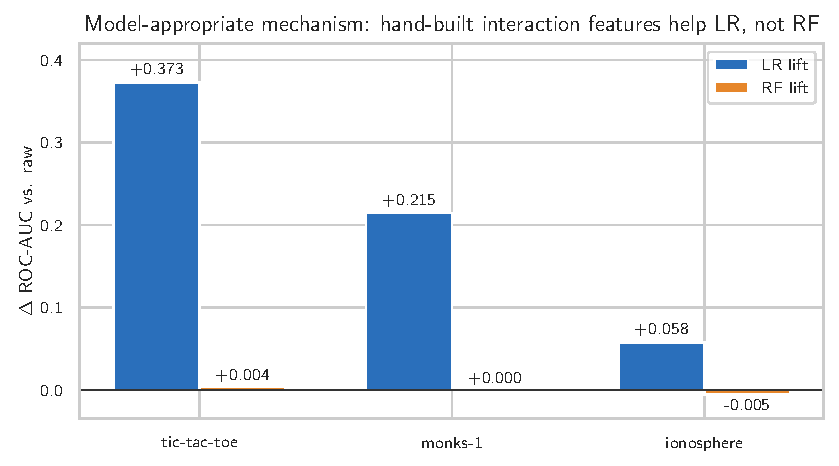
\includegraphics[width=0.8\linewidth]{figures/fig4_mechanism.pdf}
\caption{Mechanism case study on three validation datasets (not in the benchmark). Hand-constructed interaction features provide large LR gains on interaction-heavy tasks while RF remains near ceiling, illustrating why benefits can be model-appropriate rather than universal.}\label{fig:mechanism-panel}
\end{figure}


\section{Post-cutoff dataset provenance}\label{app:postcutoff-data}

Table~\ref{tab:postcutoff-data} lists the six post-cutoff tables, their Hugging Face repositories and creation dates, underlying sources and licences, sizes after preparation, and target derivations. Datasets were used as feature matrices only; free-text and most identifier columns were dropped and binary targets were derived as stated. Two retained columns are worth noting: the prediction-market table keeps a numeric market identifier and the real-estate table keeps an ordinal scrape-time code, and some generated formulas use them. Each table was fetched in June 2026. The \texttt{ImpliedData/prediction-markets} repository was public under CC BY-NC 4.0 when the table was fetched but was no longer publicly accessible on 11 October 2026, and the real-estate repository is updated continuously, so its current head differs from the table used here; the prepared feature matrices of all six tables are therefore included in the release (the prediction-market and web-tracker matrices under their original CC BY-NC 4.0 and CC BY-NC-SA 4.0 terms), so that this part of the replication remains reproducible.


\begin{table}[htbp]
\caption{Post-cutoff benchmark provenance. Sizes are rows $\times$ features after preparation (the prediction-market table is the repository's complete 40,189-row hourly candle table; its market-metadata tables were not used).}\label{tab:postcutoff-data}
\centering
\scriptsize
\begin{adjustbox}{max width=\linewidth}
\begin{tabular}{>{\raggedright\arraybackslash}p{1.9cm}>{\raggedright\arraybackslash}p{3.5cm}>{\raggedright\arraybackslash}p{3.7cm}r>{\raggedright\arraybackslash}p{1.8cm}}
\toprule
Dataset & Hugging Face repository (created) & Underlying source; licence & Size & Target \\
\midrule
clinical trials & moncefem/clinical-trials-ai-2000-2025 (2026-05-17) & ClinicalTrials.gov AI/ML trial records, 2000--2025; Apache 2.0 & \(2{,}977 \times 28\) & industry-sponsored flag \\
prediction markets & ImpliedData/prediction-markets (2026-05-17) & Polymarket/Manifold hourly candles; CC BY-NC 4.0 & \(40{,}189 \times 7\) & close above open \\
real estate & palerflavius/ro-real-estate-listings (2026-05-03) & listings scraped from imobiliare.ro; MIT & \(2{,}834 \times 7\) & price above median \\
salmonella & food-ai-nexus/salmonella-serovar-hyperspectral-spectra (2026-04-01) & \citet{papa2025rapid}, Zenodo 10.5281/zenodo.16740800; CC BY 4.0 & \(25{,}972 \times 302\) & serovar \\
web trackers & olafuraron/tracker-radar-ml (2026-03-16) & DuckDuckGo Tracker Radar with EasyPrivacy labels; CC BY-NC-SA 4.0 & \(16{,}165 \times 296\) & tracker label \\
water quality & food-ai-nexus/fecal-indicator-water-nys (2026-04-06) & PAWQ \citep{weller2020landscape,green2021integrative}, Zenodo 10.5281/zenodo.18500867; MIT & \(194 \times 94\) & E.~coli above median \\
\bottomrule
\end{tabular}
\end{adjustbox}
\end{table}

\section{Benchmark datasets}\label{app:datasets}

Table~\ref{tab:datasets} lists the 49 benchmark datasets with the OpenML dataset identifier and version that were loaded, the licence recorded on OpenML, full sizes before the 5,000-row cap, class counts, categorical-column counts as loaded, and the number of schema generators covering each dataset. Every dataset was obtained through the OpenML Python client by dataset identifier, which pins one version; the per-dataset provenance record (OpenML name, version, licence string, upload date, original source URL and citation text as published on OpenML) is released with the code as \texttt{dataset\_provenance.csv}. See Section~\ref{sec:datasets} for the three locally cached core variants and the expansion-tier selection rule.


\begin{table}[htbp]
\caption{Benchmark datasets. ``OpenML id'' and ``Ver.'' are the OpenML dataset identifier and version that were loaded (each identifier denotes one fixed version); ``Licence'' is the licence recorded on OpenML (``Public'' is an uploader assertion recorded by OpenML that no restrictive licence applies, not a formal licence; ``see source'' marks entries that name a source rather than a licence; the OpenML source description of each is in the released provenance file). Rows and features are the full table as loaded before the 5{,}000-row cap ($^{\dagger}$: local variant of the listed OpenML table, whose own listing has a different size; Section~\ref{sec:datasets}); ``Cat.'' is the number of categorical columns; ``Gen.'' is the number of schema generators with a cached linear/SVM schema for the dataset (core datasets also have tree and distance schemas from all four generators). Six core datasets (adult income, bank marketing, car evaluation, electricity, phoneme, spambase) are loaded from a local cache; for three of them (adult income, bank marketing, car evaluation) it stores the categorical columns as integer codes, which are restored to categorical columns before downstream modelling (Section~\ref{sec:protocol}); three are local variants of the listed OpenML table (Section~\ref{sec:datasets}).}\label{tab:datasets}
\centering
\scriptsize
\begin{adjustbox}{max width=\linewidth}
\begin{tabular}{llrrlrrrrr}
\toprule
Tier & Dataset & OpenML id & Ver. & Licence & Rows & Features & Classes & Cat. & Gen. \\
\midrule
core & adult\_income$^{\dagger}$ & 1590 & 2 & Public & 45{,}222 & 14 & 2 & 8 & 4 \\
core & bank\_marketing$^{\dagger}$ & 1461 & 1 & Public & 41{,}188 & 20 & 2 & 10 & 4 \\
core & blood\_transfusion & 1464 & 1 & Public & 748 & 4 & 2 & 0 & 4 \\
core & car\_evaluation & 40975 & 3 & Public & 1{,}728 & 6 & 4 & 6 & 4 \\
core & credit\_g & 31 & 1 & Public & 1{,}000 & 20 & 2 & 13 & 4 \\
core & electricity$^{\dagger}$ & 151 & 1 & Public & 38{,}474 & 7 & 2 & 0 & 4 \\
core & phoneme & 1489 & 1 & Public & 5{,}404 & 5 & 2 & 0 & 4 \\
core & pima\_diabetes & 37 & 1 & Public & 768 & 8 & 2 & 0 & 4 \\
core & qsar\_biodegradation & 1494 & 1 & Public & 1{,}055 & 41 & 2 & 0 & 4 \\
core & spambase & 44 & 1 & Public & 4{,}601 & 57 & 2 & 0 & 4 \\
\midrule
expansion & 2dplanes & 727 & 2 & Public & 40{,}768 & 10 & 2 & 0 & 3 \\
expansion & ailerons & 734 & 2 & Public & 13{,}750 & 40 & 2 & 0 & 4 \\
expansion & airlines & 42493 & 3 & Public & 26{,}969 & 7 & 2 & 5 & 4 \\
expansion & amazon\_employee\_access & 4135 & 1 & Public & 32{,}769 & 9 & 2 & 9 & 3 \\
expansion & bitcoinheist\_ransomware & 45037 & 2 & Public & 24{,}780 & 7 & 2 & 0 & 4 \\
expansion & bng\_breast\_w & 251 & 1 & Public & 39{,}366 & 9 & 2 & 0 & 4 \\
expansion & bng\_tic\_tac\_toe & 137 & 1 & Public & 39{,}366 & 9 & 2 & 9 & 2 \\
expansion & click\_prediction\_small & 1220 & 5 & Public & 39{,}948 & 9 & 2 & 0 & 4 \\
expansion & codexglue & 46682 & 1 & see source & 27{,}318 & 5 & 2 & 4 & 2 \\
expansion & coil2000\_insurance\_policies & 46916 & 1 & CC BY 4.0 & 9{,}822 & 85 & 2 & 5 & 4 \\
expansion & compass & 44162 & 3 & see source & 16{,}644 & 17 & 2 & 9 & 4 \\
expansion & customer\_churn\_classification\_nominal & 46371 & 1 & CC BY 4.0 & 35{,}000 & 24 & 2 & 0 & 4 \\
expansion & employee\_turnover\_at\_techco & 43551 & 1 & CC BY 4.0 & 34{,}452 & 9 & 2 & 0 & 4 \\
expansion & first\_order\_theorem\_proving & 1475 & 1 & Public & 6{,}118 & 51 & 6 & 0 & 4 \\
expansion & fried & 901 & 2 & Public & 40{,}768 & 10 & 2 & 0 & 4 \\
expansion & house\_16h & 821 & 2 & Public & 22{,}784 & 16 & 2 & 0 & 4 \\
expansion & house\_8l & 843 & 2 & Public & 22{,}784 & 8 & 2 & 0 & 4 \\
expansion & jungle\_chess\_2pcs\_raw\_endgame\_complete & 41027 & 1 & Public & 44{,}819 & 6 & 3 & 0 & 3 \\
expansion & kr\_vs\_kp & 3 & 1 & Public & 3{,}196 & 36 & 2 & 36 & 4 \\
expansion & law\_school\_admission\_bianry & 43890 & 2 & Public & 20{,}800 & 11 & 2 & 4 & 3 \\
expansion & led24 & 40677 & 1 & Public & 3{,}200 & 24 & 10 & 24 & 2 \\
expansion & led7 & 40678 & 1 & Public & 3{,}200 & 7 & 10 & 7 & 2 \\
expansion & loan\_approval\_status\_classification & 46526 & 1 & CC BY 4.0 & 45{,}000 & 23 & 2 & 0 & 4 \\
expansion & loan\_status & 46553 & 1 & CC BY 4.0 & 45{,}000 & 13 & 2 & 5 & 4 \\
expansion & microaggregation2 & 41671 & 1 & CC0 & 20{,}000 & 20 & 5 & 0 & 4 \\
expansion & mozilla4 & 1046 & 1 & Public & 15{,}545 & 5 & 2 & 0 & 4 \\
expansion & mushroom & 43922 & 3 & Public & 8{,}124 & 22 & 2 & 22 & 2 \\
expansion & mv & 881 & 2 & Public & 40{,}768 & 10 & 2 & 3 & 4 \\
expansion & naticusdroid & 46969 & 3 & CC BY 4.0 & 7{,}491 & 86 & 2 & 86 & 2 \\
expansion & news\_channel & 46652 & 1 & see source & 20{,}284 & 17 & 6 & 1 & 4 \\
expansion & okcupid\_stem & 45067 & 1 & Public & 26{,}677 & 13 & 3 & 11 & 1 \\
expansion & online\_shoppers & 45060 & 1 & Public & 12{,}330 & 17 & 2 & 12 & 4 \\
expansion & optdigits & 28 & 1 & Public & 5{,}620 & 64 & 10 & 0 & 3 \\
expansion & phishingwebsites & 4534 & 1 & Public & 11{,}055 & 30 & 2 & 30 & 4 \\
expansion & pol & 722 & 2 & Public & 15{,}000 & 48 & 2 & 0 & 4 \\
expansion & pricerunner & 45714 & 3 & BSD & 35{,}300 & 5 & 10 & 2 & 1 \\
expansion & splice & 46 & 1 & Public & 3{,}190 & 60 & 3 & 60 & 3 \\
expansion & taiwanese\_bankruptcy\_prediction & 46962 & 1 & CC BY 4.0 & 6{,}819 & 94 & 2 & 0 & 3 \\
expansion & volcanoes\_c1 & 1537 & 1 & Public & 28{,}626 & 3 & 5 & 0 & 4 \\
\bottomrule
\end{tabular}
\end{adjustbox}
\end{table}

\section{Core tier with all three schema families}\label{app:core-families}

The benchmark-wide analyses use the linear/SVM-family schema of each generator. On the core tier every generator also produced tree-family and distance-family schemas, giving 12 schema runs per dataset. Table~\ref{tab:core-families} reports the semantic and direct contrasts with all 12 runs averaged per dataset. The pattern matches the linear/SVM-only and benchmark-wide results: the semantic control is 10/0 for LR and KNN on ROC-AUC and 10/0 for all four models on balanced accuracy, the tree-ensemble ROC-AUC contrasts are positive but weak (RF 7/3, \(p = 0.16\); XGBoost 8/2, \(p = 0.049\)), and the direct gains are small (LR \(+0.005\), 7/3) or absent.


\begin{table}[htbp]
\caption{Core tier, all three schema families and four generators averaged per dataset ($N = 10$). Columns as in Table~\ref{tab:semantic-direct}; $p$ is the exact two-sided Wilcoxon test, whose smallest attainable value for ten datasets is 0.002.}\label{tab:core-families}
\centering
\small
\begin{adjustbox}{max width=\linewidth}
\begin{tabular}{llrrrrrrr}
\toprule
Metric & Downstream model & \(N\) & Semantic \(\Delta\) & W/L & \(p\) & Direct \(\Delta\) & W/L & \(p\) \\
\midrule
ROC-AUC & Logistic regression & 10 & +0.0115 & 10/0 & 0.002 & +0.0053 & 7/3 & 0.131 \\
ROC-AUC & KNN & 10 & +0.0632 & 10/0 & 0.002 & +0.0020 & 5/5 & 0.625 \\
ROC-AUC & Random forest & 10 & +0.0043 & 7/3 & 0.160 & -0.0011 & 4/6 & 0.625 \\
ROC-AUC & XGBoost & 10 & +0.0053 & 8/2 & 0.049 & +0.0001 & 4/6 & 0.922 \\
\midrule
Bal. accuracy & Logistic regression & 10 & +0.0135 & 10/0 & 0.002 & +0.0044 & 7/3 & 0.375 \\
Bal. accuracy & KNN & 10 & +0.0945 & 10/0 & 0.002 & +0.0219 & 6/4 & 0.105 \\
Bal. accuracy & Random forest & 10 & +0.0506 & 10/0 & 0.002 & +0.0040 & 6/4 & 0.432 \\
Bal. accuracy & XGBoost & 10 & +0.0256 & 10/0 & 0.002 & +0.0009 & 6/4 & 0.375 \\
\bottomrule
\end{tabular}
\end{adjustbox}
\end{table}

\section{Per-dataset deltas}\label{app:per-dataset}

Table~\ref{tab:per-dataset} gives the semantic-control and direct ROC-AUC deltas for every benchmark dataset and downstream model, averaged over the generators covering the dataset. Entries of \(\pm 0.000\) on mushroom, optdigits, pricerunner and similar datasets reflect raw scores at the ceiling (Appendix~\ref{app:raw-scores}).


\begin{table}[htbp]
\caption{Per-dataset ROC-AUC deltas, averaged over the generators covering each dataset (Gen.). Semantic: \texttt{raw+formula} minus \texttt{raw+permuted-formula}; direct: \texttt{raw+formula} minus \texttt{raw}.}\label{tab:per-dataset}
\centering
\scriptsize
\setlength{\tabcolsep}{3pt}
\begin{adjustbox}{max width=\linewidth}
\begin{tabular}{llrrrrrrrrr}
\toprule
& & & \multicolumn{4}{c}{Semantic $\Delta$} & \multicolumn{4}{c}{Direct $\Delta$} \\
\cmidrule(lr){4-7}\cmidrule(lr){8-11}
Tier & Dataset & Gen. & LR & KNN & RF & XGB & LR & KNN & RF & XGB \\
\midrule
core & adult\_income & 4 & +0.005 & +0.030 & -0.002 & -0.001 & +0.004 & +0.002 & +0.002 & -0.002 \\
core & bank\_marketing & 4 & +0.002 & +0.016 & -0.001 & +0.000 & +0.001 & -0.006 & +0.001 & -0.001 \\
core & blood\_transfusion & 4 & +0.026 & +0.049 & -0.036 & -0.020 & -0.000 & -0.001 & -0.004 & -0.002 \\
core & car\_evaluation & 4 & +0.008 & +0.184 & +0.006 & +0.007 & +0.003 & -0.008 & -0.000 & -0.000 \\
core & credit\_g & 4 & +0.009 & +0.091 & +0.015 & +0.019 & +0.001 & +0.033 & +0.002 & +0.000 \\
core & electricity & 4 & +0.005 & +0.089 & +0.014 & +0.013 & +0.003 & -0.001 & -0.010 & -0.003 \\
core & phoneme & 4 & +0.042 & +0.084 & +0.034 & +0.021 & +0.039 & -0.001 & +0.000 & +0.005 \\
core & pima\_diabetes & 4 & +0.014 & +0.051 & +0.013 & +0.003 & +0.003 & +0.010 & +0.006 & +0.009 \\
core & qsar\_biodegradation & 4 & +0.004 & +0.015 & +0.002 & +0.004 & -0.000 & -0.006 & -0.002 & -0.002 \\
core & spambase & 4 & +0.007 & +0.030 & +0.001 & +0.001 & +0.006 & +0.012 & -0.002 & -0.000 \\
\midrule
expansion & 2dplanes & 3 & +0.033 & +0.029 & -0.000 & -0.000 & +0.032 & +0.003 & -0.001 & -0.001 \\
expansion & ailerons & 4 & +0.000 & +0.025 & +0.007 & +0.001 & -0.000 & -0.000 & -0.000 & -0.001 \\
expansion & airlines & 4 & +0.005 & +0.024 & -0.002 & +0.009 & +0.003 & -0.020 & -0.004 & -0.005 \\
expansion & amazon\_employee\_access & 3 & +0.002 & +0.055 & +0.016 & +0.046 & +0.003 & -0.001 & +0.003 & +0.005 \\
expansion & bitcoinheist\_ransomware & 4 & +0.068 & +0.204 & +0.012 & +0.009 & +0.065 & +0.062 & -0.000 & -0.000 \\
expansion & bng\_breast\_w & 4 & +0.001 & +0.004 & -0.000 & +0.000 & +0.001 & -0.000 & -0.000 & -0.000 \\
expansion & bng\_tic\_tac\_toe & 2 & +0.008 & +0.099 & -0.000 & +0.017 & +0.007 & +0.004 & +0.004 & -0.018 \\
expansion & click\_prediction\_small & 4 & +0.034 & +0.045 & +0.006 & +0.009 & +0.022 & +0.026 & -0.006 & -0.005 \\
expansion & codexglue & 2 & +0.004 & +0.093 & +0.044 & +0.042 & -0.002 & -0.021 & +0.019 & +0.010 \\
expansion & coil2000\_insurance\_policies & 4 & +0.012 & +0.011 & +0.010 & +0.014 & +0.008 & +0.012 & +0.006 & +0.003 \\
expansion & compass & 4 & +0.008 & +0.031 & +0.039 & +0.020 & +0.006 & +0.013 & +0.007 & +0.004 \\
expansion & customer\_churn\_classification\_nominal & 4 & +0.048 & +0.043 & +0.001 & -0.001 & +0.046 & +0.024 & +0.002 & -0.001 \\
expansion & employee\_turnover\_at\_techco & 4 & +0.003 & -0.018 & +0.142 & +0.104 & -0.016 & +0.026 & +0.007 & -0.002 \\
expansion & first\_order\_theorem\_proving & 4 & +0.011 & +0.044 & -0.000 & +0.015 & +0.006 & +0.000 & -0.001 & +0.000 \\
expansion & fried & 4 & +0.064 & +0.086 & +0.024 & +0.007 & +0.063 & +0.038 & +0.017 & +0.006 \\
expansion & house\_16h & 4 & +0.027 & +0.047 & +0.001 & +0.002 & +0.025 & +0.001 & -0.002 & -0.000 \\
expansion & house\_8l & 4 & +0.023 & +0.065 & +0.002 & +0.004 & +0.022 & +0.013 & -0.002 & -0.002 \\
expansion & jungle\_chess\_2pcs\_raw\_endgame\_complete & 3 & +0.035 & +0.098 & +0.048 & +0.042 & +0.033 & -0.009 & +0.025 & +0.022 \\
expansion & kr\_vs\_kp & 4 & +0.000 & +0.054 & +0.001 & +0.000 & +0.000 & -0.012 & +0.000 & +0.000 \\
expansion & law\_school\_admission\_bianry & 3 & +0.000 & +0.022 & +0.000 & +0.000 & +0.000 & -0.014 & +0.000 & +0.000 \\
expansion & led24 & 2 & +0.002 & +0.069 & -0.004 & +0.001 & -0.000 & +0.018 & -0.003 & +0.002 \\
expansion & led7 & 2 & +0.001 & +0.036 & -0.004 & +0.006 & -0.000 & -0.004 & -0.000 & -0.003 \\
expansion & loan\_approval\_status\_classification & 4 & +0.004 & +0.017 & +0.001 & +0.001 & +0.003 & +0.010 & -0.002 & -0.001 \\
expansion & loan\_status & 4 & +0.003 & +0.052 & +0.002 & +0.001 & +0.002 & +0.006 & -0.001 & -0.001 \\
expansion & microaggregation2 & 4 & +0.020 & +0.040 & -0.001 & +0.014 & +0.013 & -0.001 & -0.005 & +0.002 \\
expansion & mozilla4 & 4 & +0.031 & +0.139 & +0.017 & +0.012 & +0.026 & +0.015 & -0.001 & +0.002 \\
expansion & mushroom & 2 & +0.000 & +0.000 & +0.000 & +0.000 & +0.000 & -0.000 & +0.000 & +0.000 \\
expansion & mv & 4 & +0.000 & +0.023 & +0.001 & +0.000 & +0.000 & +0.001 & +0.000 & -0.000 \\
expansion & naticusdroid & 2 & +0.000 & +0.005 & -0.002 & +0.001 & -0.000 & -0.003 & -0.000 & -0.000 \\
expansion & news\_channel & 4 & +0.013 & +0.054 & +0.016 & +0.017 & +0.007 & +0.013 & +0.004 & +0.006 \\
expansion & okcupid\_stem & 1 & -0.000 & +0.066 & -0.000 & +0.002 & -0.000 & +0.009 & +0.002 & -0.001 \\
expansion & online\_shoppers & 4 & +0.027 & +0.117 & +0.009 & -0.001 & +0.024 & +0.055 & +0.007 & -0.003 \\
expansion & optdigits & 3 & +0.000 & +0.000 & +0.000 & +0.000 & +0.000 & +0.000 & -0.000 & +0.000 \\
expansion & phishingwebsites & 4 & +0.000 & +0.018 & -0.000 & +0.003 & -0.000 & -0.001 & -0.000 & -0.000 \\
expansion & pol & 4 & +0.037 & +0.025 & +0.002 & +0.001 & +0.037 & +0.003 & +0.000 & +0.000 \\
expansion & pricerunner & 1 & +0.000 & +0.050 & +0.000 & +0.000 & -0.000 & -0.000 & -0.000 & +0.000 \\
expansion & splice & 3 & +0.000 & +0.025 & -0.000 & -0.000 & +0.000 & +0.018 & -0.001 & -0.000 \\
expansion & taiwanese\_bankruptcy\_prediction & 3 & +0.001 & +0.024 & -0.004 & +0.003 & -0.001 & +0.004 & -0.000 & +0.001 \\
expansion & volcanoes\_c1 & 4 & +0.038 & +0.035 & -0.008 & -0.027 & -0.024 & +0.003 & +0.022 & -0.025 \\
\bottomrule
\end{tabular}
\end{adjustbox}
\end{table}

\section{Raw baseline scores}\label{app:raw-scores}

Table~\ref{tab:raw-scores} reports the raw-feature ROC-AUC of each downstream model on each benchmark dataset. Nine datasets (bng\_breast\_w, car evaluation, kr\_vs\_kp, law school admission, mushroom, mv, optdigits, pol, pricerunner) have raw XGBoost at or above 0.995, so the absence of a tree-ensemble gain there is a ceiling effect; the datasets carrying the LR direct gain are those where raw LR trails the tree ensembles the most (Section~\ref{sec:direct}).


\begin{table}[htbp]
\caption{Raw-feature ROC-AUC per dataset and downstream model (generator-averaged evaluation split; the raw matrix is shared across generators).}\label{tab:raw-scores}
\centering
\scriptsize
\begin{adjustbox}{max width=\linewidth}
\begin{tabular}{llrrrr}
\toprule
Tier & Dataset & LR & KNN & RF & XGB \\
\midrule
core & adult\_income & 0.912 & 0.895 & 0.910 & 0.923 \\
core & bank\_marketing & 0.937 & 0.897 & 0.936 & 0.941 \\
core & blood\_transfusion & 0.764 & 0.730 & 0.702 & 0.703 \\
core & car\_evaluation & 0.981 & 0.971 & 0.997 & 0.998 \\
core & credit\_g & 0.793 & 0.736 & 0.800 & 0.793 \\
core & electricity & 0.819 & 0.838 & 0.888 & 0.891 \\
core & phoneme & 0.805 & 0.914 & 0.953 & 0.936 \\
core & pima\_diabetes & 0.823 & 0.795 & 0.820 & 0.797 \\
core & qsar\_biodegradation & 0.914 & 0.905 & 0.926 & 0.925 \\
core & spambase & 0.972 & 0.955 & 0.986 & 0.989 \\
\midrule
expansion & 2dplanes & 0.922 & 0.970 & 0.981 & 0.985 \\
expansion & ailerons & 0.952 & 0.913 & 0.940 & 0.953 \\
expansion & airlines & 0.625 & 0.624 & 0.645 & 0.654 \\
expansion & amazon\_employee\_access & 0.747 & 0.666 & 0.762 & 0.703 \\
expansion & bitcoinheist\_ransomware & 0.704 & 0.806 & 0.913 & 0.915 \\
expansion & bng\_breast\_w & 0.997 & 0.994 & 0.997 & 0.998 \\
expansion & bng\_tic\_tac\_toe & 0.755 & 0.813 & 0.813 & 0.859 \\
expansion & click\_prediction\_small & 0.620 & 0.581 & 0.646 & 0.655 \\
expansion & codexglue & 0.796 & 0.647 & 0.694 & 0.673 \\
expansion & coil2000\_insurance\_policies & 0.688 & 0.636 & 0.724 & 0.737 \\
expansion & compass & 0.733 & 0.711 & 0.789 & 0.761 \\
expansion & customer\_churn\_classification\_nominal & 0.809 & 0.807 & 0.874 & 0.875 \\
expansion & employee\_turnover\_at\_techco & 0.660 & 0.527 & 0.684 & 0.674 \\
expansion & first\_order\_theorem\_proving & 0.703 & 0.768 & 0.823 & 0.823 \\
expansion & fried & 0.915 & 0.930 & 0.968 & 0.980 \\
expansion & house\_16h & 0.888 & 0.907 & 0.940 & 0.944 \\
expansion & house\_8l & 0.893 & 0.909 & 0.941 & 0.944 \\
expansion & jungle\_chess\_2pcs\_raw\_endgame\_complete & 0.809 & 0.900 & 0.929 & 0.948 \\
expansion & kr\_vs\_kp & 0.993 & 0.982 & 0.999 & 0.999 \\
expansion & law\_school\_admission\_bianry & 1.000 & 0.983 & 1.000 & 1.000 \\
expansion & led24 & 0.950 & 0.915 & 0.949 & 0.940 \\
expansion & led7 & 0.956 & 0.934 & 0.941 & 0.954 \\
expansion & loan\_approval\_status\_classification & 0.954 & 0.934 & 0.963 & 0.967 \\
expansion & loan\_status & 0.951 & 0.937 & 0.963 & 0.967 \\
expansion & microaggregation2 & 0.700 & 0.667 & 0.747 & 0.767 \\
expansion & mozilla4 & 0.873 & 0.902 & 0.968 & 0.966 \\
expansion & mushroom & 1.000 & 1.000 & 1.000 & 1.000 \\
expansion & mv & 0.999 & 0.987 & 0.999 & 1.000 \\
expansion & naticusdroid & 0.978 & 0.974 & 0.976 & 0.982 \\
expansion & news\_channel & 0.746 & 0.702 & 0.751 & 0.763 \\
expansion & okcupid\_stem & 0.779 & 0.736 & 0.779 & 0.793 \\
expansion & online\_shoppers & 0.885 & 0.845 & 0.908 & 0.922 \\
expansion & optdigits & 0.999 & 0.998 & 1.000 & 0.999 \\
expansion & phishingwebsites & 0.985 & 0.984 & 0.991 & 0.992 \\
expansion & pol & 0.940 & 0.987 & 0.997 & 0.998 \\
expansion & pricerunner & 1.000 & 1.000 & 1.000 & 1.000 \\
expansion & splice & 0.991 & 0.971 & 0.994 & 0.994 \\
expansion & taiwanese\_bankruptcy\_prediction & 0.910 & 0.857 & 0.927 & 0.941 \\
expansion & volcanoes\_c1 & 0.792 & 0.762 & 0.830 & 0.882 \\
\bottomrule
\end{tabular}
\end{adjustbox}
\end{table}

\section{Second judgment model}\label{app:judgment-v4pro}

As a robustness check on the judgment null of Section~\ref{sec:per-row-judgments-add-no-reliable-value-beyond-formulas}, the same incremental contrast was computed for the 93 core schema runs whose per-row judgments were produced by DeepSeek-V4-Pro (coverage 3 to 12 of the 12 cells per dataset; the remaining 15 V4-Pro runs were not completed and 12 cells have no V4-Pro judgments). Table~\ref{tab:judgment-v4pro} shows the same picture as the DeepSeek-Reasoner runs: every ROC-AUC increment is within \(\pm 0.002\) of zero (LR \(-0.0005\), 1/9; KNN \(-0.0019\), 4/6; RF \(+0.0020\), 4/6; XGBoost \(+0.0002\), 2/8) and every balanced-accuracy increment is negative with three or four wins out of ten; no cell reaches significance. These runs are excluded from the main analysis only so that every judgment cell in Table~\ref{tab:judgment} shares one judgment model; they are produced by \texttt{scripts/expansion/judgment\_second\_model.py} from the stored results.

\begin{table}[htbp]
\caption{Second judgment model: incremental effect of DeepSeek-V4-Pro per-row judgment features beyond deterministic formulas on the ten core datasets (93 completed schema runs; coverage per dataset 3 to 12 of 12 cells, averaged per dataset before testing). Columns as in Table~\ref{tab:judgment}; $p$ is the exact two-sided Wilcoxon test over datasets.}\label{tab:judgment-v4pro}
\centering
\small
\begin{tabular}{llrrrrr}
\toprule
Metric & Downstream model & \(N\) & Mean \(\Delta\) & W/L/T & Cliff's \(\delta\) & \(p\) \\
\midrule
ROC-AUC & Logistic regression & 10 & -0.0005 & 1/9/0 & -0.80 & 0.0645 \\
ROC-AUC & KNN & 10 & -0.0019 & 4/6/0 & -0.20 & 0.3223 \\
ROC-AUC & Random forest & 10 & +0.0020 & 4/6/0 & -0.20 & 0.9219 \\
ROC-AUC & XGBoost & 10 & +0.0002 & 2/8/0 & -0.60 & 0.2754 \\
\midrule
Bal. accuracy & Logistic regression & 10 & -0.0004 & 3/7/0 & -0.40 & 0.3750 \\
Bal. accuracy & KNN & 10 & -0.0032 & 3/7/0 & -0.40 & 0.1602 \\
Bal. accuracy & Random forest & 10 & -0.0009 & 3/7/0 & -0.40 & 0.3223 \\
Bal. accuracy & XGBoost & 10 & -0.0023 & 4/6/0 & -0.20 & 0.1934 \\
\bottomrule
\end{tabular}
\end{table}


\section{Protocol details}\label{app:protocol-details}

\subsection*{Protocol details}

\paragraph{Schema summary and schema sizes.}

The summary also carries the dataset's registry name (for example \texttt{adult\_income}), the target column name, the number of design rows and, for categorical columns, the number of distinct values and the count of each of the ten most frequent values; Section~\ref{sec:anon} replaces the first two. The generator is asked for a fixed schema of 12 features. All 120 core schemas and 125 of the 131 expansion schemas have exactly 12 features; the six exceptions are truncated responses described in Section~\ref{sec:scale-of-evaluation}. The schemas contain 10.1 deterministic formula features per schema on average over the 120 core schemas (10.2 for their linear/SVM family) and 9.7 on the expansion datasets, range 1 to 11; the remainder are per-row judgment specifications (one to five on the core tier, zero to nine on the expansion tier, where they are never materialized; Section~\ref{sec:judgment}).

\paragraph{Judgment generation.}

Judgments were produced for the ten core datasets by DeepSeek-Reasoner in batches of 25 rows per call; all 12 schema runs per core dataset have a judgment matrix, so the judgment comparison covers the full core grid. A second set of judgment runs with DeepSeek-V4-Pro (93 completed matrices and 15 partially filled runs) is excluded from the main analysis so that every judgment cell shares one judgment model; Appendix~\ref{app:judgment-v4pro} reports the same contrast on the completed runs. No judgments were generated for the expansion datasets.

\paragraph{Declared value range.}

The declared range of a feature is the \texttt{value\_range} interval the generator returns for it in the schema; the materialized formula column and the parsed judgment values are clipped to this interval, and the random control draws uniform values over the same interval (the range is immaterial after standardization and for tree models).

\paragraph{Random-expression templates and sampling.}

The expressions are sampled from the vocabulary the LLM formulas use (logarithms, \(z\)-scores, min--max scaling, squares and square roots, ratios, products, sums, differences, shares, threshold and two-way indicators, three-way buckets, and category indicators), using only the design-split column statistics the generators received (means, standard deviations, minima, maxima, and the most frequent categories). An expression that is constant or undefined on the design split is redrawn, and the declared value range is the design-split range. Materialization, range clipping, cross-validation folds, downstream models, and column permutation are identical to those applied to the LLM formulas. Five random schemas are drawn per cell, seeded by the cell and the draw index, and every reported random-expression score is the mean over the five draws.

\paragraph{Categorical encoding of the cached core datasets.}

The local cache of adult income, bank marketing, and car evaluation stores their categorical columns as 8-bit integer codes, and the schema generators received these columns summarized as numeric (mean, standard deviation, minimum, maximum), so their formulas reference the codes. The evaluation keeps the formulas exactly as written, computing them on the codes, but restores the columns to categoricals before downstream modelling, so the raw block is mode-imputed and one-hot encoded as for every other dataset; the random, permuted, and judgment matrices of these runs share the same rows and encoding. An earlier version of this evaluation passed the codes to the downstream models as ordinal integers, which weakened the raw LR and KNN baselines on the three datasets and inflated the formula gains there, most visibly on car evaluation; every number in this paper uses the one-hot encoding.

\paragraph{Row cap and design splits for schema generation.}

On the core tier the 5,000-row cap was applied to adult income, bank marketing and electricity, while phoneme, with 5,404 rows, was evaluated uncapped. The schema generators for the core datasets received the column-level summary of a 20--30\% design split of the full, uncapped dataset (for nine Claude Sonnet 4.6 cells on blood transfusion, credit-g, pima diabetes, and QSAR biodegradation, of the full dataset); because the 5,000-row cap nests inside that split, the summary statistics for adult income, bank marketing, and electricity also cover the rows later used for evaluation. Only distributional statistics and the class balance are exposed, never row-level labels, and Section~\ref{sec:leakage} checks that this overlap does not inflate the effects. The expansion schemas were generated from the column-level summary of a stratified 30\% design split (seed 42) of the full, uncapped dataset; the 5,000-row evaluation cap is drawn afterwards, so for the 35 expansion datasets with more than 5,000 rows the summary statistics also cover rows that later serve as evaluation rows, exactly as for the three capped core datasets, and only for the four expansion datasets with at most 5,000 rows (kr\_vs\_kp, led7, led24, splice) are the design and evaluation rows disjoint. As on the core tier, only distributional statistics and the class balance were exposed, and the check of Section~\ref{sec:leakage} bounds the effect of this overlap.

\paragraph{Multiplicity across tables.}

As a global check, Benjamini-Hochberg over the 48 dataset-level tests of Tables~\ref{tab:semantic-direct} and~\ref{tab:random-expression} leaves every cell reported as significant below \(q = 0.05\) (largest 0.019); Holm over all 48 retains every semantic effect (RF at 0.044), the LR direct gain, the LR, KNN, and RF LLM-minus-random-expression contrasts, and all excess-semantic cells, but not the KNN direct gain (either metric), the balanced-accuracy RF direct gain, or the ROC-AUC random-expression-versus-raw cells for LR and XGBoost, which we therefore describe as fragile. Holm over the 16 per-generator semantic cells of Table~\ref{tab:generators} leaves all of them below 0.05 (largest 0.026).


\section{Schema and run provenance}\label{app:provenance}

\subsection*{Schema and run provenance}

\paragraph{Expansion tier composition and coverage.}

The 39 datasets range from 3,190 to 45,000 rows and from 3 to 94 raw features, 11 are multiclass (3 to 10 classes), and 20 contain categorical columns. Each expansion dataset has the linear/SVM-family schema of every generator that produced one: 24 of the 39 are covered by all four generators, seven by three (2dplanes, amazon employee access, jungle chess, law school admission, optdigits, splice, Taiwanese bankruptcy), six by two (bng\_tic\_tac\_toe, codexglue, led7, led24, mushroom, naticusdroid), and two by one (okcupid\_stem, pricerunner). The 131 expansion-tier runs come from 48, 44, 40 and 39 datasets covered by GPT-5.5 Pro, Gemini 3.1 Pro Preview, Claude Opus 4.7 and Claude Sonnet 4.6 respectively, counting the core datasets. For 13 schema cells on seven datasets whose column names are not valid Python identifiers (for GPT-5.5 Pro: amazon employee access, bng\_tic\_tac\_toe, led7, led24, mushroom, naticusdroid, phishingwebsites; for Gemini: the same set without amazon employee access), the generator saw column names sanitized to valid identifiers and the same renaming is applied to the evaluation rows before the formulas are materialized.

\paragraph{Response accounting.}

The schema cache holds 174 raw generator responses for the core datasets, 150 of them from the four benchmark generators, of which 16 failed JSON parsing or formula validation (Claude Sonnet 4.6: 10, Gemini 3.1 Pro Preview: 4, Claude Opus 4.7: 2, GPT-5.5 Pro: 0); the remaining 24 responses (7 failures) come from two earlier Gemini versions tried in a May 2026 pilot on four core datasets and are not part of the benchmark. Twelve Claude Sonnet 4.6 cells on those four datasets have two or three valid cached schemas, generated from different design-split summaries on 9 May and 30 May 2026; for these cells the pipeline used the first file returned by a directory listing, a rule fixed before any evaluation that never consults a result, and all candidate files are released. Every other cell has exactly one valid schema. The expansion schemas are cached generator responses from 3 June 2026 under the same prompt, feature budget, and design-split summary protocol (the prompt hashes of the cached files are reproduced by the current prompt builder); they were evaluated offline on 8 September 2026 without any further LLM call. Six expansion responses (Gemini 3.1 Pro Preview on splice, kr\_vs\_kp, and phishingwebsites; GPT-5.5 Pro on mushroom, phishingwebsites, and naticusdroid) were truncated before the JSON closed; the complete feature objects that could be decoded (1 to 9 formula features and no judgment specification) were kept as the schema, which accounts for all but two of the runs with fewer than five formula columns, and their formulas pass the same validator at materialization.

\paragraph{Judgment-feature audit.}

Per-row judgment features are evaluated as an incremental addition on all 120 core runs. A judgment-feature audit of the 226 stored judgment features across these runs (\texttt{scripts/audit\_judgment\_signal.py}) found no missing values: the median feature takes 109 distinct values (quartiles 16 to 402), three features are near-constant (one value covering at least 80\% of rows), 14 have more than half of their values at a declared bound, and the judgment columns alone reach ROC-AUC 0.66 with logistic regression (median 0.65, range 0.47 to 0.83 over the 120 runs; above 0.60 in 93 runs), so they encode row-level signal. A looser boundary warning, which fires whenever a single value equals a declared endpoint, is raised for 217 of the 226 features but does not indicate degenerate outputs.

\paragraph{Constant-column scan.}

Across the 251 runs no materialized formula column is entirely missing; 25 columns in 15 runs are constant on the evaluation rows (for example a monetary-to-frequency ratio that is exactly 250 on blood transfusion, or sums of a permutation-coded block on microaggregation2), and five runs materialize fewer than five non-constant formula columns (Gemini on codexglue and splice; GPT-5.5 Pro on mushroom, naticusdroid and pricerunner). All runs are kept.

\paragraph{Leakage-equivalence check.}

Because the core schemas were generated from summaries of uncapped design splits (Section~\ref{sec:protocol}), a leakage-equivalence check compares the same Claude Sonnet 4.6 and Gemini 3.1 Pro schemas evaluated prospectively (the 80\% complement of a 20\% design split, seed 42, with no row cap, hence larger evaluation sets; for the 40 of the 60 Claude Sonnet 4.6 and Gemini 3.1 Pro schemas that were generated from that 20\% split the evaluation rows are disjoint from the summarized rows, while 11 schemas were generated from a 30\% split and 9 from the full dataset) against the cached core evaluation, on the 54 overlapping cells (9 datasets, LR/RF/KNN, two metrics). The mean absolute difference in cached-versus-prospective deltas is 0.0050, with signed cached-minus-prospective difference \(+0.0023\) (largest for KNN balanced accuracy, \(+0.014\)). The two evaluation modes therefore look broadly similar at this aggregation level; the check bounds the effect of the summary-statistics overlap on the raw-to-formula deltas rather than comparing two schema-generation regimes. The cached side averages every stored run of a dataset, including the DeepSeek-V4-Pro duplicates that re-evaluate the same formula matrices.

\paragraph{Generator settings and compute.}

Schema generation sent temperature 0 to Gemini, Claude Sonnet, and DeepSeek, omitted it for the GPT-5.5 Pro and Claude Opus 4.7 reasoning endpoints, requested reasoning effort high from GPT-5.5 Pro, set no extended-thinking parameter for the other generators (Gemini 3.1 Pro Preview reasons at its API default), used JSON output mode where available (OpenAI, Gemini, DeepSeek), and used output budgets of 16,384 tokens for GPT-5.5 Pro and 8,192 tokens otherwise; the \texttt{reasoning: max\_available} entries in the released model configuration are not transmitted to the Anthropic or Gemini APIs. Table~\ref{tab:models} lists the API identifiers, endpoints, settings, and query dates; the stored responses record the alias passed to the API, token counts, and text, but not the provider's resolved snapshot identifier. All downstream evaluations ran on one Apple Silicon workstation (10 cores, 24 GB): the four-generator expansion tier took about three hours, the classical baselines on the expansion datasets about three hours, and the random-expression control about 25 minutes on five worker processes. One schema is drawn per generator, family, and dataset cell and cached by prompt hash, so the reported means carry no schema-sampling variance.

\begin{table}[tbp]
\caption{Language-model endpoints, settings, and query windows. Identifiers are the strings passed to the provider APIs (\texttt{configs/llm\_models.yaml}); dates are those of the cached responses. OpenAI documents \texttt{gpt-5.5-pro-2026-04-23} as the snapshot behind the \texttt{gpt-5.5-pro} alias; the other aliases are not version-pinned by their providers.}\label{tab:models}
\centering
\scriptsize
\setlength{\tabcolsep}{4pt}
\begin{tabular}{>{\raggedright\arraybackslash}p{1.3cm}>{\raggedright\arraybackslash}p{1.6cm}>{\raggedright\arraybackslash}p{2.8cm}>{\raggedright\arraybackslash}p{2.0cm}>{\raggedright\arraybackslash}p{2.8cm}>{\raggedright\arraybackslash}p{3.0cm}}
\toprule
Role & Name in text & API identifier & Endpoint & Settings & Queried \\
\midrule
Schema generator & GPT-5.5 Pro & \texttt{gpt-5.5-pro} & OpenAI Responses API & reasoning effort high; no temperature; 16,384 output tokens; JSON mode & core 1 June 2026; expansion 3 June; post-cutoff 8 June (one retry 21 June); anonymized 21 June \\
Schema generator & Gemini 3.1 Pro Preview & \texttt{gemini-3.1-pro-}\allowbreak\texttt{preview} & Google Generative Language API & temperature 0; 8,192 tokens; JSON mode; default thinking & core 31 May to 1 June 2026; expansion 3 June; post-cutoff 8 June \\
Schema generator & Claude Opus 4.7 & \texttt{claude-opus-4-7} & Anthropic Messages API & no temperature; 8,192 tokens & core 31 May to 1 June 2026; expansion 3 June \\
Schema generator & Claude Sonnet 4.6 & \texttt{claude-sonnet-4-6} & Anthropic Messages API & temperature 0; 8,192 tokens & core 9 May and 30 May to 1 June 2026; expansion 3 June \\
Judgment filler & DeepSeek-Reasoner & \texttt{deepseek-}\allowbreak\texttt{reasoner} & DeepSeek chat completions & temperature 0; JSON mode; 25 rows per call & 1 to 2 June 2026 \\
Judgment filler (Appendix~\ref{app:judgment-v4pro}) & DeepSeek-V4-Pro & \texttt{deepseek-v4-pro} & DeepSeek chat completions & temperature 0; JSON mode; 25 rows per call & 1 to 3 June 2026 \\
\bottomrule
\end{tabular}
\end{table}

\paragraph{Benchmark table licences and maintenance.}

The derived artifacts released under CC BY 4.0 are the schemas, responses, judgment outputs, scores, and statistics; the stored feature matrices are regenerable from the cached schemas. The OpenML benchmark tables are fetched by dataset identifier, which pins one version; the release redistributes only the six locally cached core tables (the three variants of Section~\ref{sec:datasets} and verbatim copies of car evaluation, phoneme, and spambase, all recorded as public on OpenML), the prepared post-cutoff tables of Table~\ref{tab:postcutoff-data} under their own licences (included because one repository is no longer public and another is updated continuously; Appendix~\ref{app:postcutoff-data}), and, inside every stored feature matrix, the raw evaluation-split columns of the dataset concerned. The authors maintain the repository, accept issues and corrections, and record changes in a changelog; a datasheet-style description of the benchmark (composition, preparation, intended uses, licences, hosting, and maintenance) accompanies the supplementary material.


\section{Additional tables and figures}\label{app:extra-tables}

\subsection*{Random-feature and permuted-formula controls}

Table~\ref{tab:random-controls} shows the random-feature controls.


\begin{table}[tbp]
\caption{Random-feature and permuted-formula controls versus raw features on all 49 datasets (ROC-AUC, generator-averaged). Every count-matched control degrades every model; W/L counts datasets on which the control beats raw.}\label{tab:random-controls}
\centering
\small
\begin{adjustbox}{max width=\linewidth}
\begin{tabular}{lrrrrrrr}
\toprule
Downstream model & \(N\) & Random-formula \(-\) raw & W/L & Random-all \(-\) raw & W/L & Permuted \(-\) raw & W/L \\
\midrule
Logistic regression & 49 & -0.0038 & 4/44 & -0.0065 & 0/48 & -0.0044 & 3/45 \\
KNN & 49 & -0.0474 & 2/47 & -0.0585 & 2/47 & -0.0443 & 2/47 \\
Random forest & 49 & -0.0083 & 9/38 & -0.0110 & 10/37 & -0.0067 & 11/36 \\
XGBoost & 49 & -0.0127 & 3/43 & -0.0148 & 3/44 & -0.0085 & 5/41 \\
\bottomrule
\end{tabular}
\end{adjustbox}
\end{table}

\subsection*{Where the semantic effect is largest}

The largest effects come from datasets with interaction-heavy or ratio-friendly structure (bitcoinheist ransomware, fried, customer churn, phoneme, volcanoes and pol for LR; bitcoinheist, car evaluation, mozilla4 and online shoppers for KNN), and the effect vanishes for every model only where every raw model is already at the ceiling (mushroom and optdigits, where all four raw models are at or above ROC-AUC 0.998; pricerunner is equally saturated but keeps a KNN effect; Appendix~\ref{app:per-dataset}).

\subsection*{Critical-difference diagrams}

Figure~\ref{fig:cd} shows the critical-difference diagrams summarized in Section~\ref{sec:model-appropriate-interaction}. Under the standard Demšar convention (lower average rank is better), ranks are averaged over the 49 datasets among the raw, formula, permuted-formula, random-formula, and random-all variants, and the critical difference is from the Nemenyi post-hoc test at \(\alpha = 0.05\) with \(k = 5\) treatments and \(N = 49\) (CD \(= 0.87\)). For LR, \texttt{raw+formula} attains the best average rank (1.37) ahead of raw features (1.90), with the permuted and random controls more than one CD behind (3.63 to 4.43); the formula-versus-raw gap is itself within one CD. For XGBoost raw features rank first (1.70) with \texttt{raw+formula} second (2.03) and the three controls again more than one CD behind. KNN mirrors LR (formula 1.47, raw 1.71) and RF mirrors XGBoost (raw 2.12, formula 2.39). For LR, KNN and XGBoost the aligned formula matrix is separated from its permuted copy by more than the critical difference; for RF the gap (2.90 versus 2.39) is within it, consistent with RF's small semantic effect.

\begin{figure}[tbp]
\centering
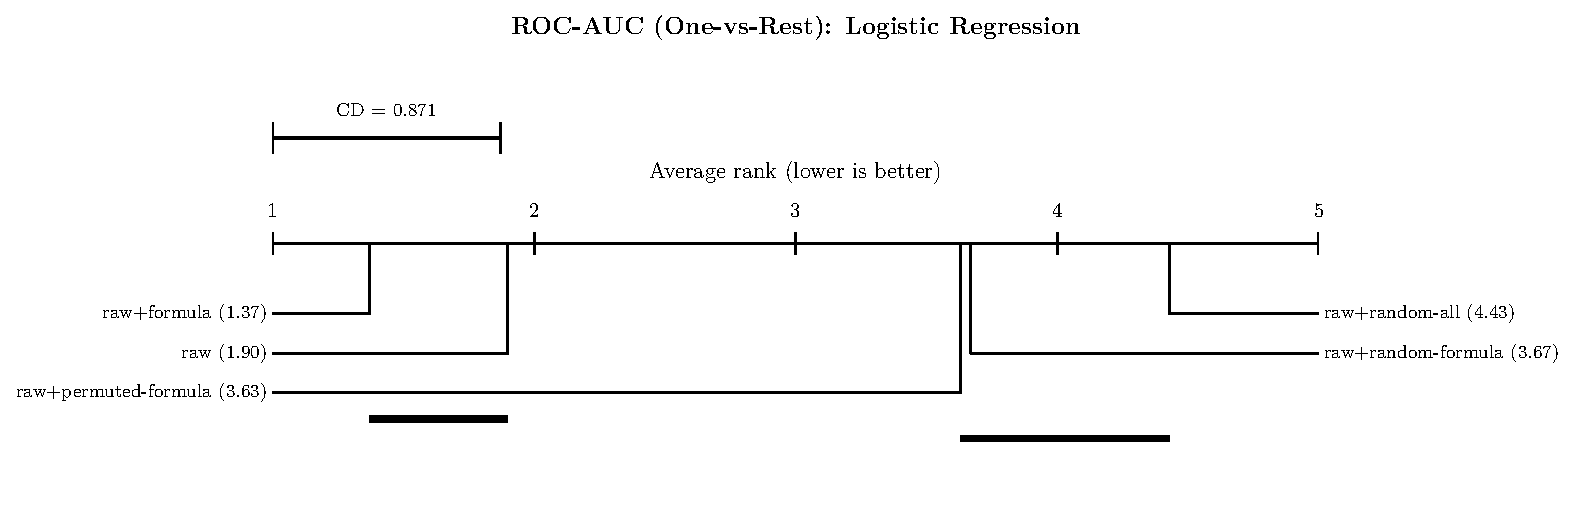
\includegraphics[width=0.85\linewidth]{figures/fig3a_cd_lr.pdf}\\[4pt]
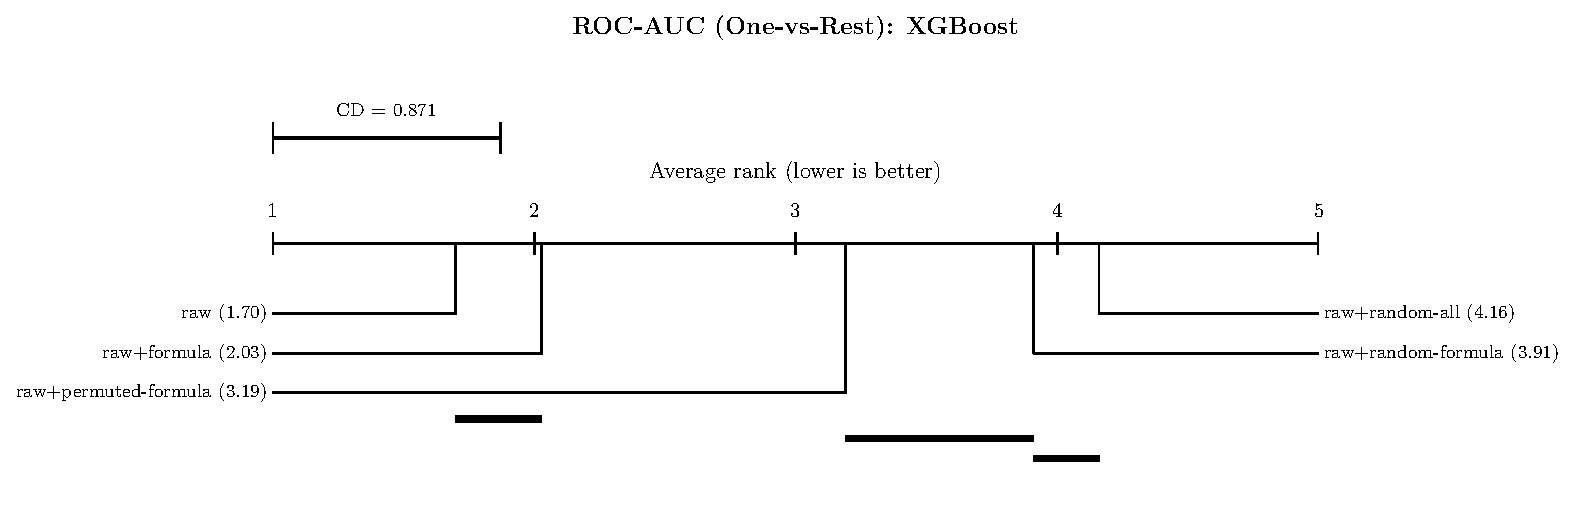
\includegraphics[width=0.85\linewidth]{figures/fig3b_cd_xgboost.pdf}
\caption{Critical-difference diagrams for ROC-AUC with logistic regression (top) and XGBoost (bottom) over the 49 datasets (Nemenyi test, $\alpha = 0.05$, $k = 5$, CD $= 0.87$; lower average rank is better). Formula features rank first for LR and second behind raw features for XGBoost; in both cases the permuted-formula and random controls are more than one critical difference behind the aligned formula matrix.}\label{fig:cd}
\end{figure}

\subsection*{Per-generator results}

Table~\ref{tab:generators} reports the semantic and direct contrasts for each generator separately, on the datasets it covers (48 for GPT-5.5 Pro, 44 for Gemini 3.1 Pro Preview, 40 for Claude Opus 4.7, 39 for Claude Sonnet 4.6).

\begin{table}[tbp]
\caption{Semantic control and direct effect by schema generator (linear/SVM schemas, ROC-AUC, one generator at a time on the datasets it covers). Columns as in Table~\ref{tab:semantic-direct}.}\label{tab:generators}
\centering
\small
\begin{adjustbox}{max width=\linewidth}
\begin{tabular}{llrrrrrrr}
\toprule
Generator & Downstream model & \(N\) & Semantic \(\Delta\) & W/L & \(p\) & Direct \(\Delta\) & W/L & \(p\) \\
\midrule
GPT-5.5 Pro & Logistic regression & 48 & +0.0150 & 46/1 & $<$0.001 & +0.0108 & 33/14 & $<$0.001 \\
 & KNN & 48 & +0.0520 & 44/4 & $<$0.001 & +0.0076 & 29/19 & 0.015 \\
 & Random forest & 48 & +0.0099 & 32/14 & 0.003 & +0.0026 & 20/26 & 0.931 \\
 & XGBoost & 48 & +0.0098 & 37/8 & $<$0.001 & +0.0009 & 21/24 & 0.929 \\
\midrule
Gemini 3.1 Pro Preview & Logistic regression & 44 & +0.0134 & 42/2 & $<$0.001 & +0.0081 & 33/11 & $<$0.001 \\
 & KNN & 44 & +0.0476 & 42/2 & $<$0.001 & +0.0052 & 22/22 & 0.154 \\
 & Random forest & 44 & +0.0083 & 26/17 & 0.026 & +0.0010 & 20/23 & 0.853 \\
 & XGBoost & 44 & +0.0081 & 33/10 & $<$0.001 & -0.0002 & 18/25 & 0.603 \\
\midrule
Claude Opus 4.7 & Logistic regression & 40 & +0.0193 & 37/2 & $<$0.001 & +0.0136 & 33/6 & $<$0.001 \\
 & KNN & 40 & +0.0548 & 40/0 & $<$0.001 & +0.0108 & 27/13 & 0.004 \\
 & Random forest & 40 & +0.0083 & 31/8 & $<$0.001 & +0.0013 & 17/22 & 0.961 \\
 & XGBoost & 40 & +0.0090 & 32/7 & $<$0.001 & -0.0002 & 15/24 & 0.225 \\
\midrule
Claude Sonnet 4.6 & Logistic regression & 39 & +0.0144 & 35/3 & $<$0.001 & +0.0098 & 33/5 & $<$0.001 \\
 & KNN & 39 & +0.0512 & 38/1 & $<$0.001 & +0.0068 & 28/11 & 0.006 \\
 & Random forest & 39 & +0.0095 & 29/9 & $<$0.001 & +0.0019 & 20/18 & 0.646 \\
 & XGBoost & 39 & +0.0065 & 34/4 & $<$0.001 & -0.0009 & 17/21 & 0.528 \\
\bottomrule
\end{tabular}
\end{adjustbox}
\end{table}

\subsection*{Classical baseline settings}

We ran three classical automated feature-engineering baselines on exactly the DASEF protocol: the same cap-then-split rows (the evaluation split is row-identical to the stored DASEF matrices, asserted at run time), the same 5\(\times\)2 CV, and the same four downstream models. The baselines are pairwise polynomial interactions (interaction-only products, top 12 selected by mutual information), OpenFE (top 12 generated features), and autofeat (one feature-engineering step with log, square-root, and square transforms). To mirror the LLM generator, which sees only a summary of the 30\% design split, each classical system is fitted on the design split (where it may use labels) and its features are then materialized on the evaluation split; no evaluation-split label is used outside the cross-validation training folds. This is stricter than the common practice of selecting features on the full evaluation data, and it leaves the classical systems only a few hundred design rows on the smallest datasets, a limitation of the matched protocol rather than of the systems. OpenFE was run in its first stage only, with two data blocks, at least 100 candidate features, one repeat, and seed 42, and its transform step sees the design and evaluation feature values (never labels) together because its group-by operators require both; the polynomial selector uses mutual information with random state 42; and the classical systems operate on a numeric encoding of the inputs (ordinal category codes and median imputation fitted on the design split), while the downstream models receive the raw columns plus the generated columns. Polynomial features cover all 49 datasets. OpenFE covers 47: it crashes natively on bng\_tic\_tac\_toe and mushroom (reproducibly, inside its own worker pool), and those two datasets are excluded from its rows. Autofeat returns additional features on 19 of the 49 datasets and is compared on those. On balanced accuracy OpenFE is ahead for KNN (\(+0.023\) versus \(+0.013\), \(p = 0.004\)) and RF (\(+0.012\) versus \(+0.008\), \(p = 0.016\)).

\subsection*{Post-cutoff replication: generation settings, knowledge cutoffs, and scope}

Schemas are generated only from each dataset's design split (a 20\% design split with no row cap, versus the 30\% split and 5,000-row cap of the main benchmark) using GPT-5.5 Pro and Gemini 3.1 Pro Preview; we evaluate the raw, formula, and random-control matrices, add the column-permuted formula control post hoc from the stored formula matrices (each generated column independently row-permuted, seed 42, evaluated with the same folds), and do not generate per-row judgments. Unlike the main benchmark, which uses the linear/SVM family only, the post-cutoff analysis uses all three schema families of both generators: the completed runs of a dataset (six, or five for prediction markets) are averaged per dataset before the Wilcoxon test, for the permuted, random-formula, and direct contrasts alike. The GPT-5.5 Pro distance-family cell on clinical trials required a second generation call after the first response failed JSON parsing. Four of the six repackage records that were publicly available before the model cutoffs (the underlying water-quality, hyperspectral, tracker, and clinical-trial data), so the control addresses memorization of these specific tables and of feature recipes published for them, not all prior exposure to the domains. Memorized formulas for these specific tables are not a plausible explanation of the effect here, because the tables did not exist in this form when the models were trained (OpenAI documents a 1 December 2025 knowledge cutoff for GPT-5.5 Pro\footnote{\url{https://developers.openai.com/api/docs/models/gpt-5.5-pro}, accessed 11 October 2026; the page lists \texttt{gpt-5.5-pro-2026-04-23} as the default snapshot.}; Google publishes no knowledge cutoff for Gemini 3.1 Pro Preview, but its public-preview release date of 19 February 2026 precedes the creation of all six tables\footnote{\url{https://ai.google.dev/gemini-api/docs/models/gemini-3.1-pro-preview} and \url{https://docs.cloud.google.com/vertex-ai/generative-ai/docs/models/gemini/3-1-pro}, accessed 11 October 2026.}). In Table~\ref{tab:postcutoff} the 5/1 semantic cells have \(p = 0.063\) for KNN ROC-AUC and RF balanced accuracy and \(p = 0.16\) for RF ROC-AUC, and all four models are positive in mean for both metrics. The weaker count-matched noise control (\texttt{raw+random-formula}) gives the same picture (ROC-AUC: LR \(+0.042\), RF \(+0.019\), KNN \(+0.084\), XGBoost \(+0.021\); 5/6 or 6/6 in every cell). The injected random-feature controls degrade KNN, RF, and XGBoost relative to raw features and leave LR roughly unchanged, so the gap is not a dimensionality artifact. With only six datasets these effects are a supportive replication rather than a powered confirmation; grouped cross-validation and redefined targets are future work.

\subsection*{Anonymized-column control: prompt contents, remaining cues, and like-for-like comparison}

Column names are replaced by generic tokens (\texttt{x001}, \texttt{x002}, \ldots), the dataset name and the target column name are replaced by generic tokens (the OpenML identifier is never part of a prompt), and the distributional summary (dtype, mean/std/min/max, missing rate, number of distinct values, category frequencies, row count, class balance) is retained. Two identifying cues remain: the class-label strings in the class-balance entry (such as \texttt{>50K}, \texttt{tested\_positive}, or \texttt{spam}) and, for credit-g, the categorical value strings, so the control removes column semantics rather than every cue to dataset identity. Like for like, the anonymized effect is not smaller than the same generator's named-column effect, so on these ten datasets column semantics add no measurable increment beyond the domain-agnostic component; the four-generator named-column average on the same ten datasets is similar (LR \(+0.012\), the mean of the core rows of Table~\ref{tab:per-dataset}), but that comparison mixes generators. The anonymized control uses a single generator, so it is a directional check rather than a full re-run of the multi-generator benchmark.

\subsection*{Random-expression control: limitations in detail}

The random-expression control draws five random schemas per cell from a fixed vocabulary with uniform template and column choices and averages their scores; a stronger label-free baseline, such as search over the same vocabulary with a validation criterion, might narrow the LLM-minus-random gap further, and the classical baselines of Section~\ref{sec:classical} are the label-using version of that comparison; its templates reference at most two columns, whereas many LLM formulas combine three or more, and LLM formula columns are clipped to the generator's declared range while random expressions use the design-split range.

\subsection*{Downstream-awareness diagnostic}

The pipeline included schema prompts targeted to model families such as linear/SVM, tree, and distance-based models. Across the core tier (10 datasets, 4 generators, 4 downstream models, 160 matched-versus-best-mismatched ROC-AUC comparisons on the raw-to-formula contrast), the matched prompt family beat the better of the two mismatched families in 57 comparisons and lost in 103 (44 of 120 when restricted to LR, RF, and KNN; 48 of 160 on balanced accuracy), consistent with chance (the expected win rate against the better of two alternatives under the null is one third). Model-family prompting does not reliably produce better-matched features in these experiments, which is also why the benchmark-wide analyses use a single family; a larger core tier may reveal family-specific effects.



\end{document}
